\section{Experiment Results and Analysis}
\label{sec:experiment_results}

In this section, we answers the four questions in Section~\ref{sec:experimental_scheme} one by one with experiments.
Without otherwise mentioned, when we report the training time per epoch of a GNN, we measure the training time of 50 epoches, exclude the epoches with abnormal training time \footnote{During the training of some epoches, there were extra profiling overheads from NVIDIA Nsight Systems and GC pauses from the Python interpreter that significantly increased the training time. Assume Q1 and Q3 are the 25\% and 75\% quantiles of the training time of 50 epoches, respectively. We regard the epoches with the training time \emph{outside} the range of $[Q1 - 1.5 * (Q3-Q1), Q3 + 1.5 * (Q3-Q1)]$ as abnormal epoches.} and report the average time of the remaining epoches.

\subsection{Effects of Hyper-parameters on Performance}
\label{sec:effects_of_hyper-parameters_on_performance}

To verify the time complexity analysis in \tablename~\ref{tab:gnn_overview_edge} and \tablename~\ref{tab:gnn_overview_vertex}, we first compare the training time of the four GNNs on the same dataset.
\figurename~\ref{fig:exp_absolute_training_time} shows the wall-clock training time per epoch of the GNNs on the real-world datasets.
The ranking of the training time was GaAN $\gg$ GAT $>$ GGNN $>$ GCN in all cases.
Since the real-world graphs had more edges than edges ($m > n$), the time complexity of the edge computation affected more than the vertex computation.
The ranking was consistent with the time complexity analysis.

\begin{figure}
    \centering
    \subfloat[\texttt{pub}\label{fig:exp_absolute_training_time_pubmed}]{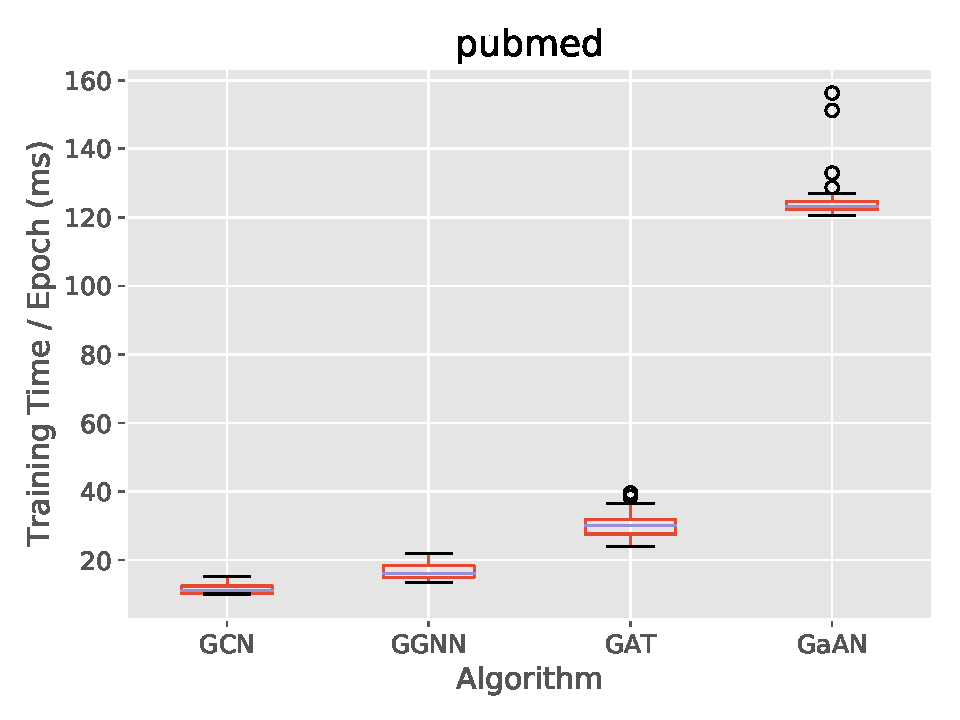
\includegraphics[height=4cm]{figs/experiments/exp_absolute_training_time_comparison_pubmed.pdf}}
    \subfloat[\texttt{aph}\label{fig:exp_absolute_training_time_amazon-photo}]{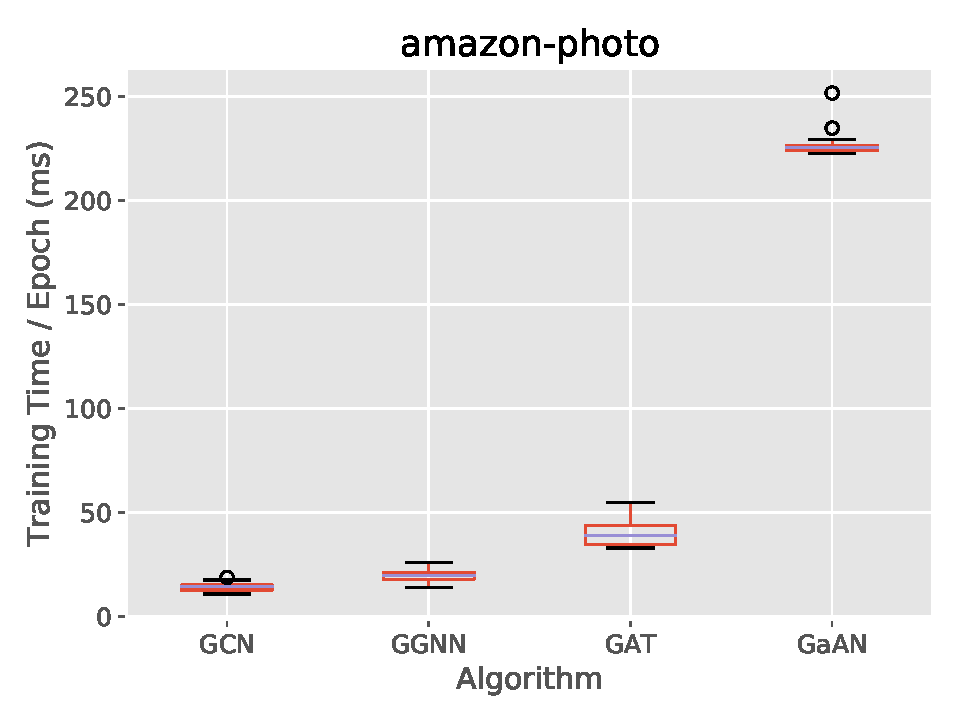
\includegraphics[height=4cm]{figs/experiments/exp_absolute_training_time_comparison_amazon-photo.pdf}}
    \subfloat[\texttt{cph}\label{fig:exp_absolute_training_time_coauthor-physics}]{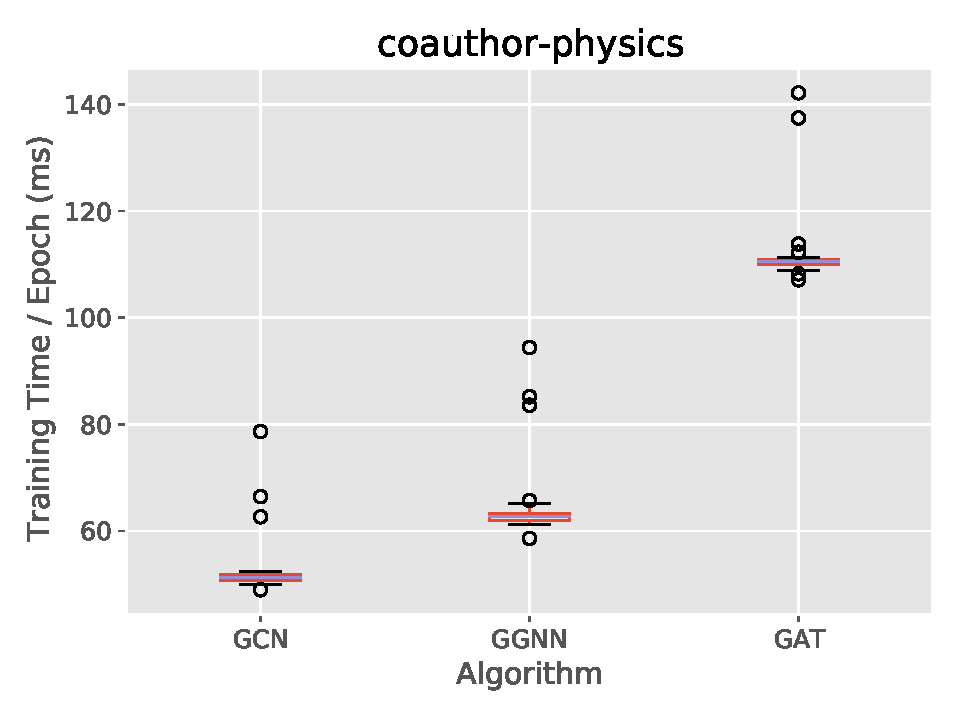
\includegraphics[height=4cm]{figs/experiments/exp_absolute_training_time_comparison_coauthor-physics.pdf}} \\
    \subfloat[\texttt{amc}\label{fig:exp_absolute_training_time_amazon-computers}]{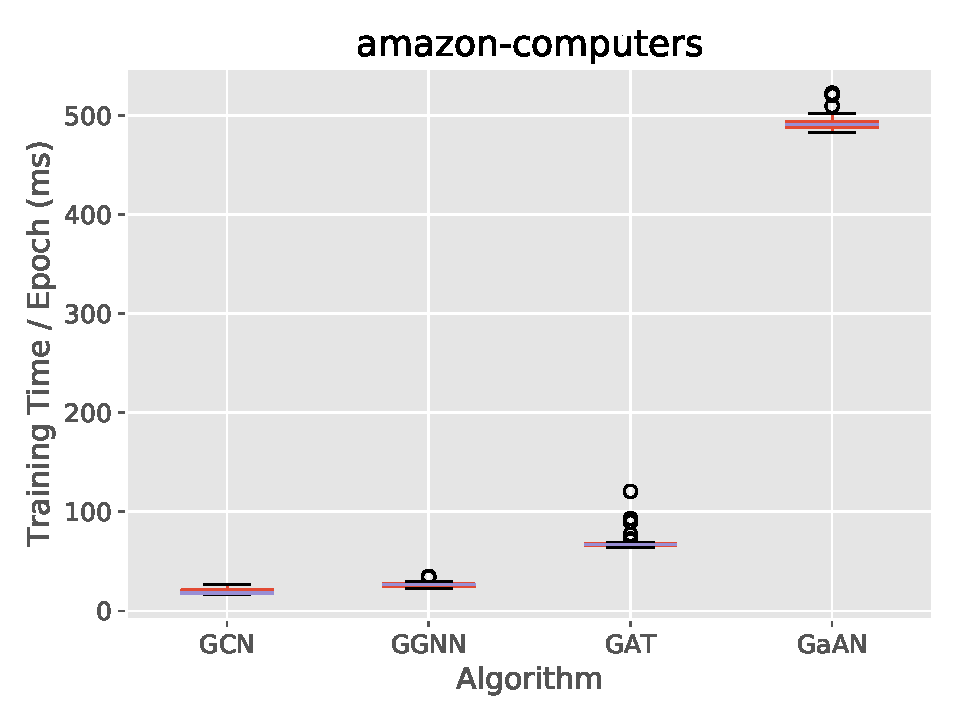
\includegraphics[height=4cm]{figs/experiments/exp_absolute_training_time_comparison_amazon-computers.pdf}}
    \subfloat[\texttt{fli}\label{fig:exp_absolute_training_time_flickr}]{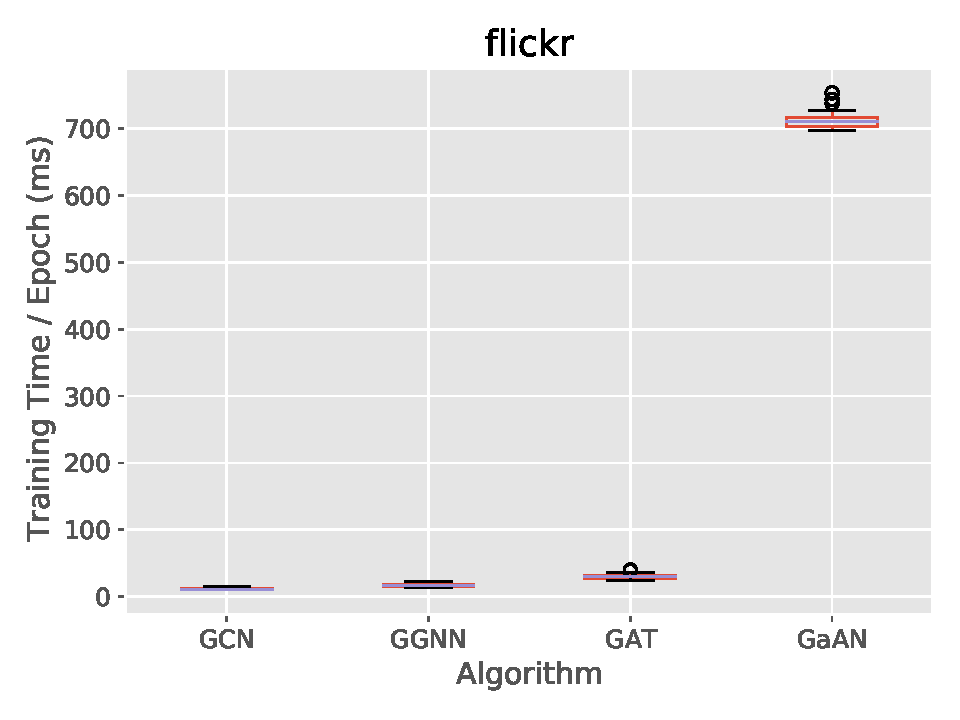
\includegraphics[height=4cm]{figs/experiments/exp_absolute_training_time_comparison_flickr.pdf}}
    \subfloat[\texttt{cam}\label{fig:exp_absolute_training_time_com-amazon}]{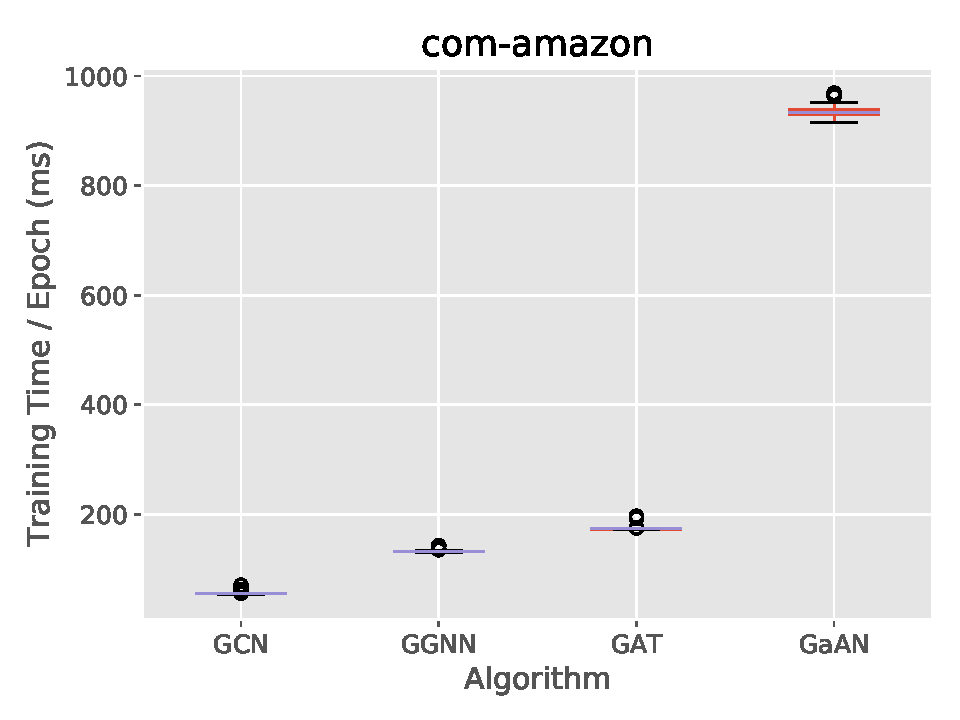
\includegraphics[height=4cm]{figs/experiments/exp_absolute_training_time_comparison_com-amazon.pdf}}
    \caption{Distribution of the wall-clock training time of 50 epoches on different datasets. GaAN crashed due to out of memory exception on the \texttt{cph} dataset.}
    \label{fig:exp_absolute_training_time}
\end{figure}

Fixing other hyper-parameters, the time complexity of $\phi$/$\gamma$ is linear to each hyper-parameter separately, according to the analysis in \tablename~\ref{tab:gnn_overview_edge} and \tablename~\ref{tab:gnn_overview_vertex}.
If we increase one of the hyper-parameters, the training time should also increase linearly.
In order to verify the linearity, we measured the training time of each GNN with varying hyper-parameters in \figurename~\ref{fig:exp_hyperparameter_on_vertex_edge_phase_time}.

\begin{figure}
    \centering
    \subfloat[GCN\label{fig:exp_hyperparameter_on_vertex_edge_phase_time_gcn}]{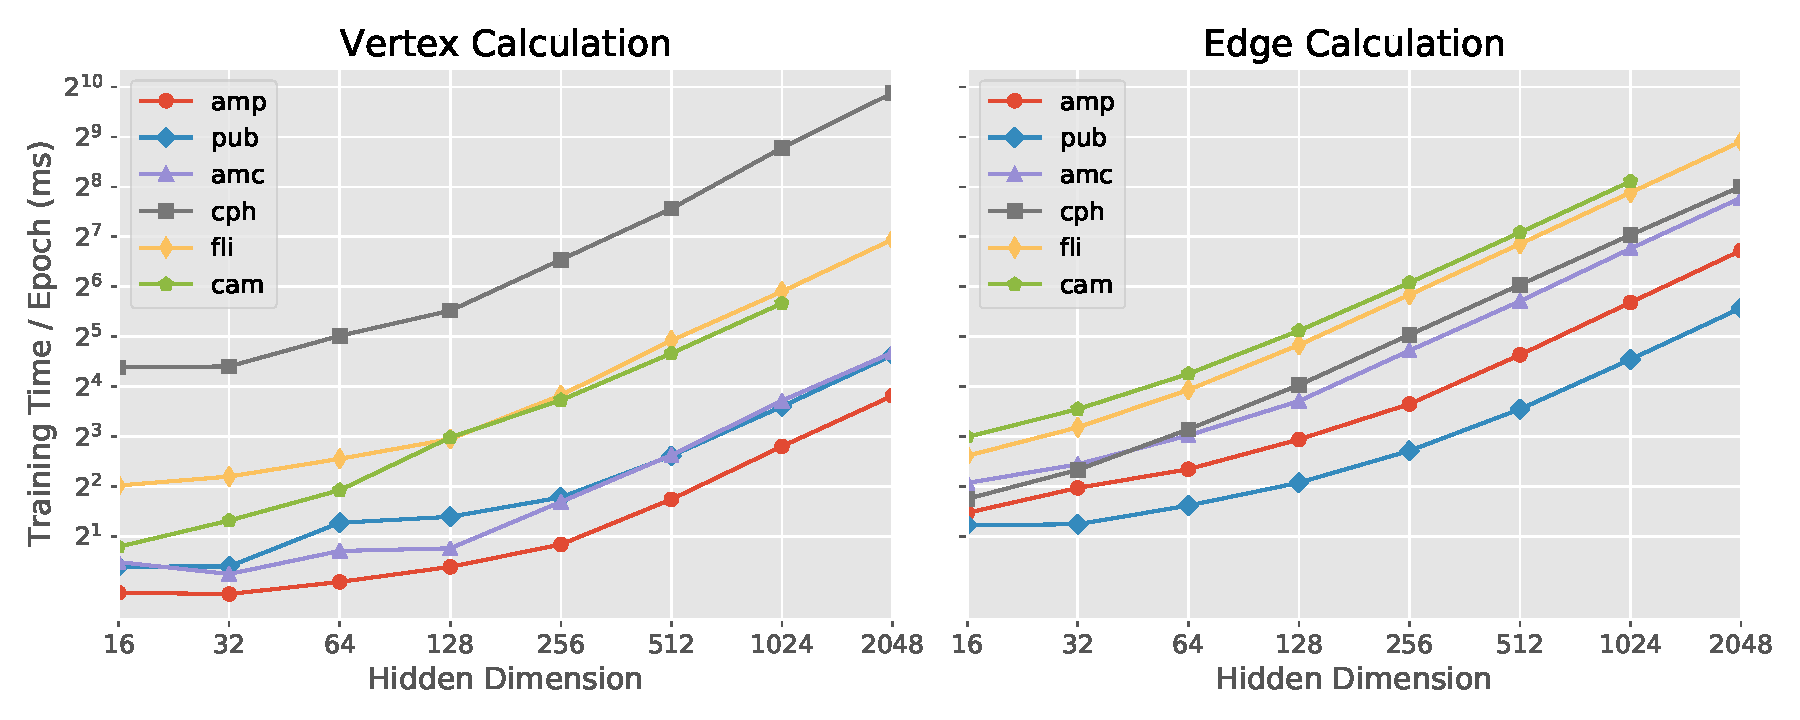
\includegraphics[height=3cm]{figs/experiments/exp_hyperparameter_on_vertex_edge_phase_time_gcn.pdf}}
    %
    \subfloat[GGNN\label{fig:exp_hyperparameter_on_vertex_edge_phase_time_ggnn}]{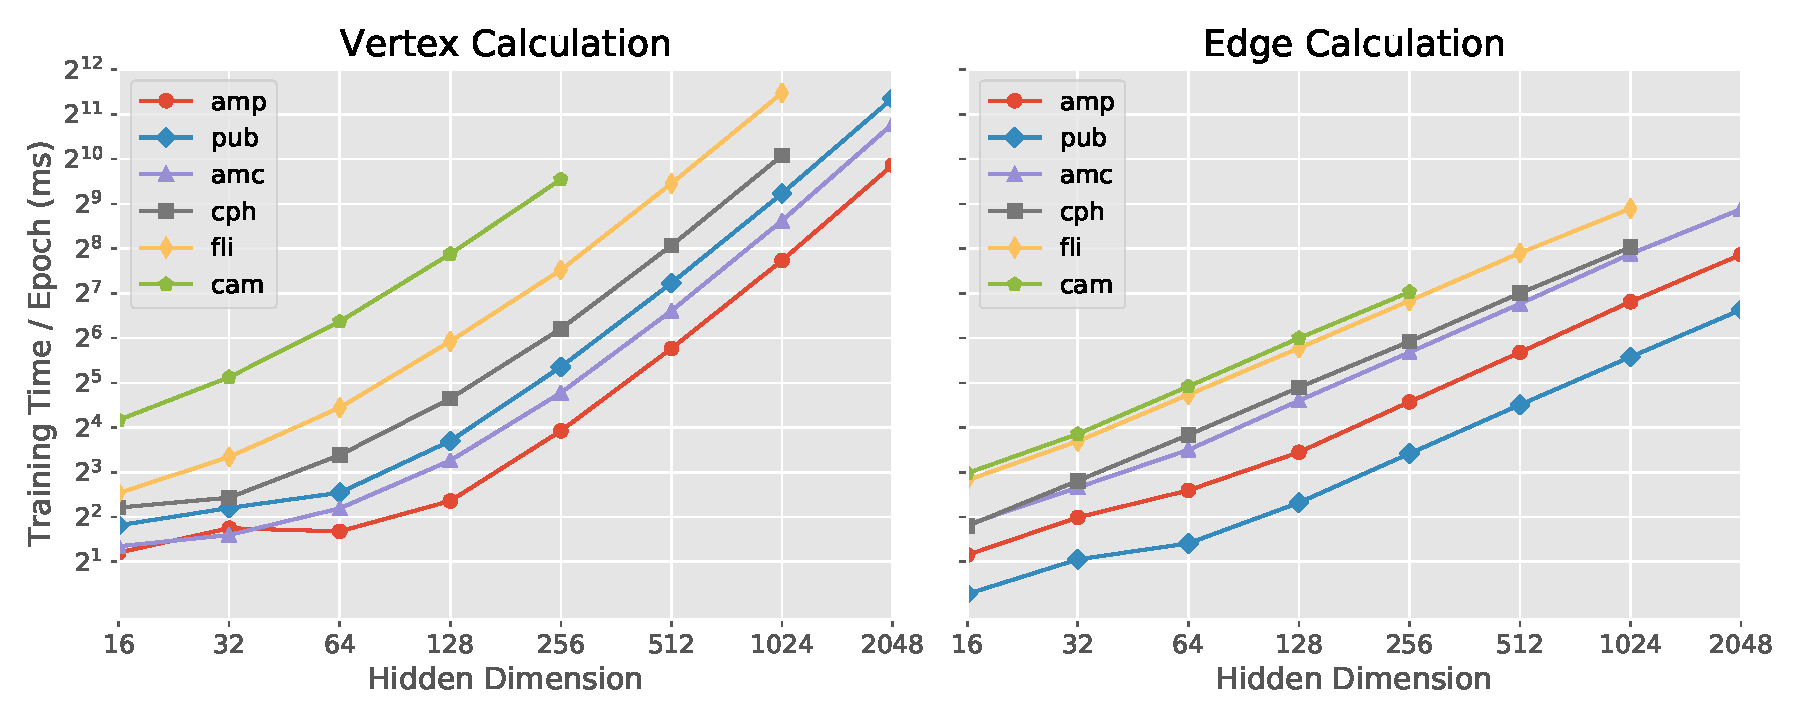
\includegraphics[height=3cm]{figs/experiments/exp_hyperparameter_on_vertex_edge_phase_time_ggnn.pdf}}

    \subfloat[GAT]{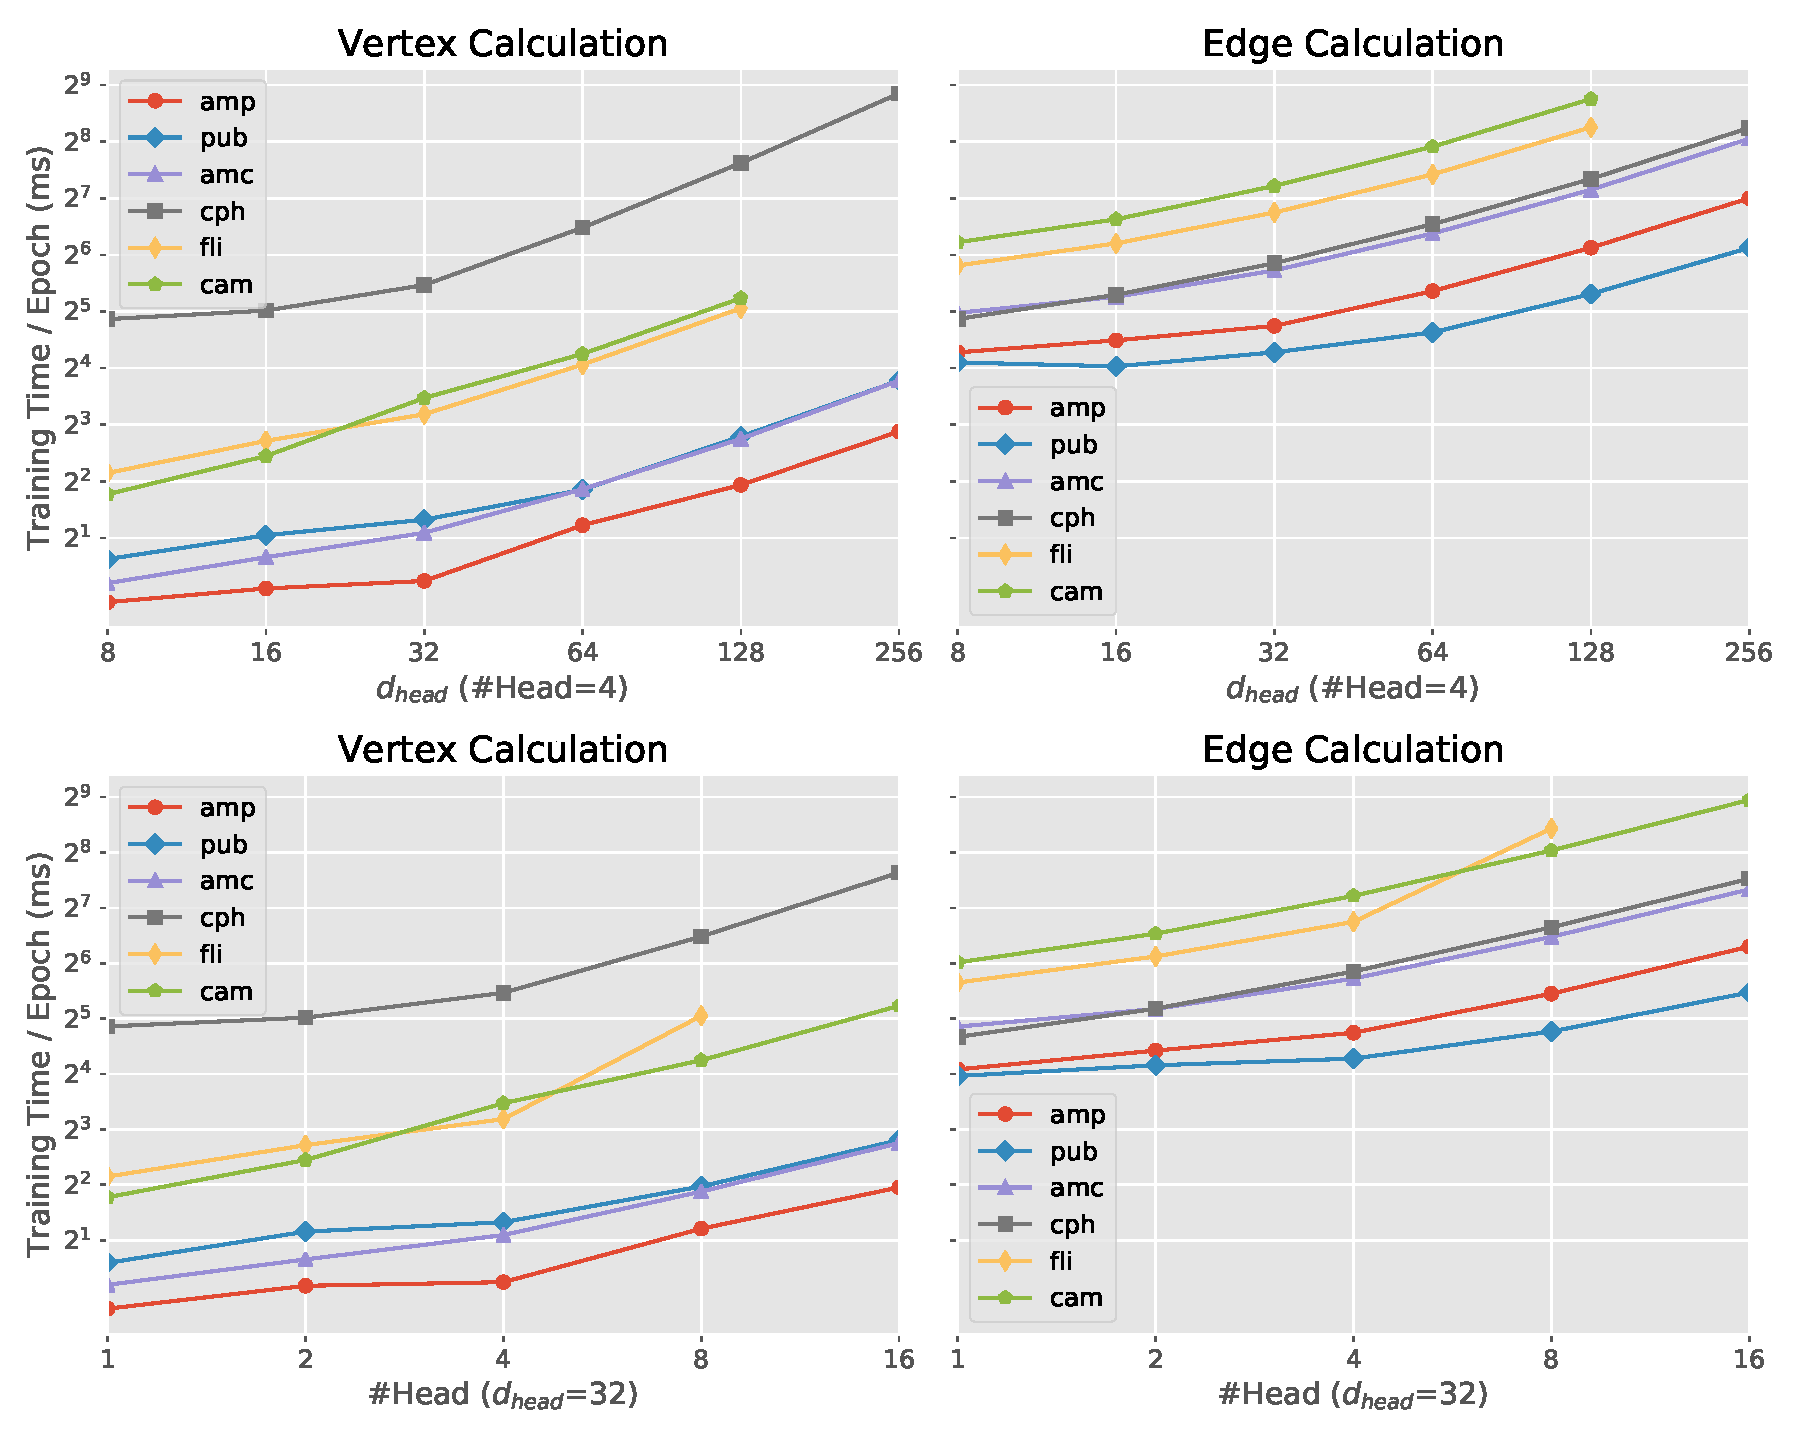
\includegraphics[height=6cm]{figs/experiments/exp_hyperparameter_on_vertex_edge_phase_time_gat.pdf}}

    \subfloat[GaAN]{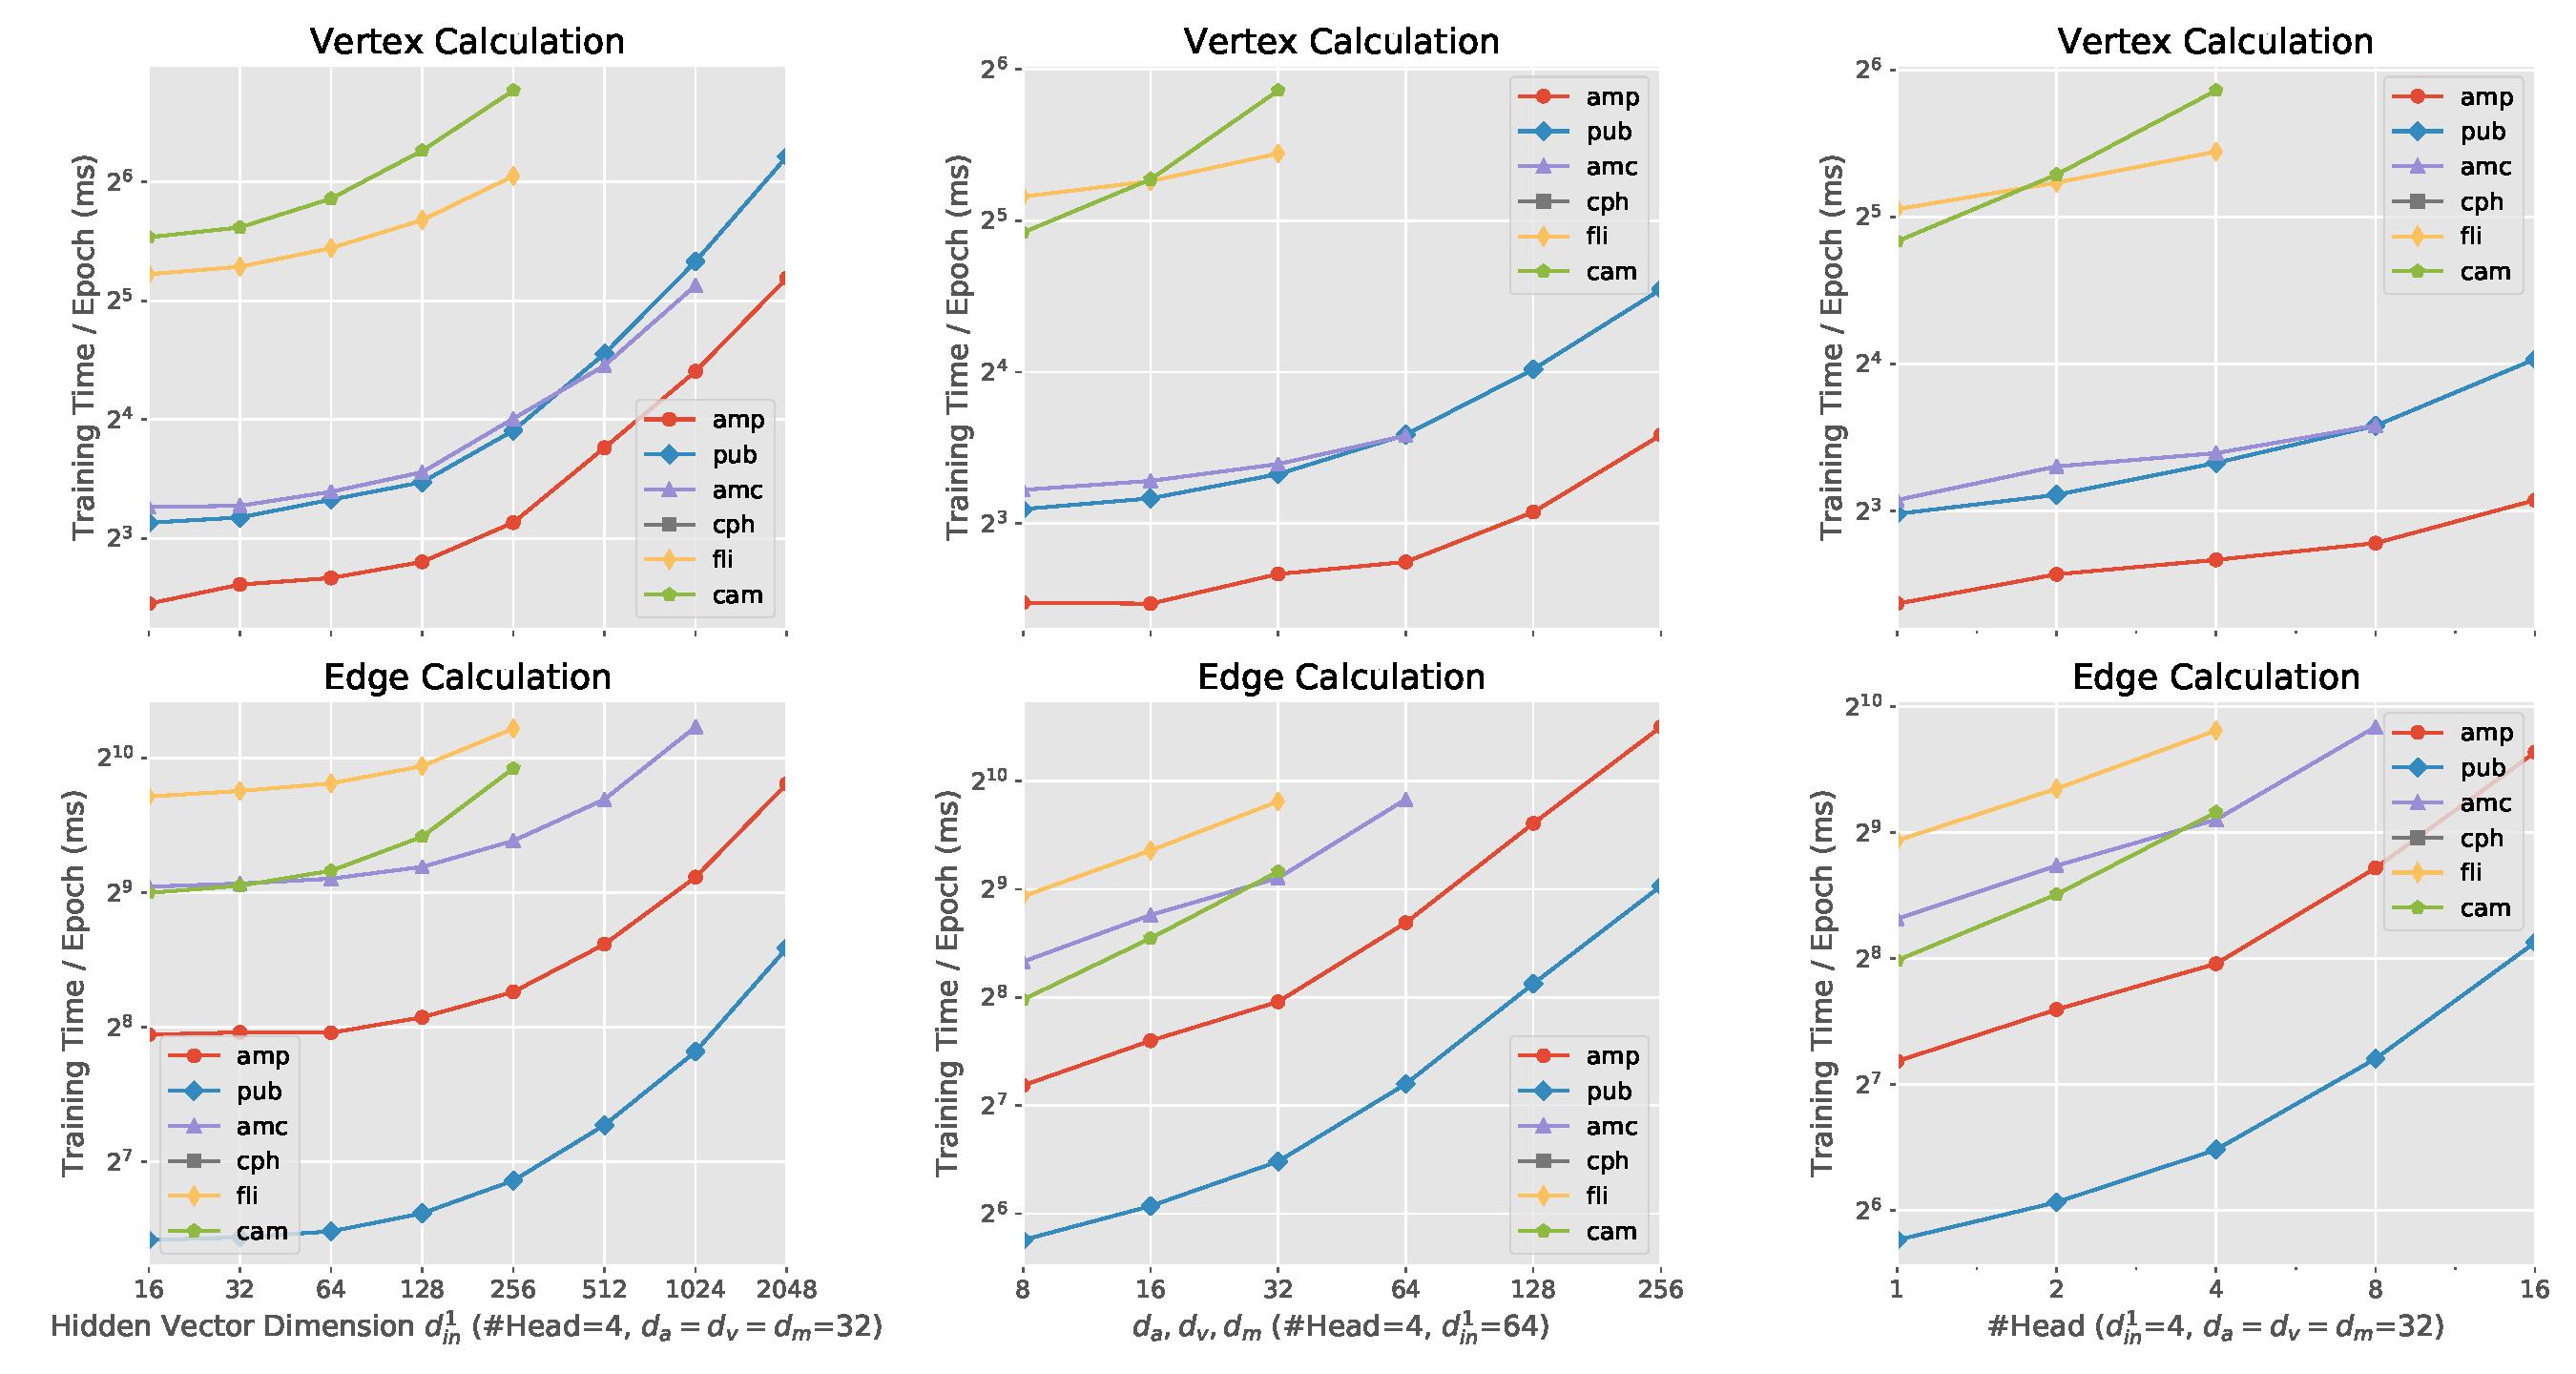
\includegraphics[height=6cm]{figs/experiments/exp_hyperparameter_on_vertex_edge_phase_time_gaan.pdf}}

    \caption{Effects of hyper-parameters on vertex/edge calculation time.}
    \label{fig:exp_hyperparameter_on_vertex_edge_phase_time}
\end{figure}


For GCN (\figurename~\ref{fig:exp_hyperparameter_on_vertex_edge_phase_time_gcn}) and GGNN (\figurename~\ref{fig:exp_hyperparameter_on_vertex_edge_phase_time_ggnn}), the only modifiable hyper-parameter is the hidden dimension $dim(\boldsymbol{h}^1)$, as $dim(\boldsymbol{h}^0)$ and $dim(\boldsymbol{h}^2)$ is determined by the dataset with $dim(\boldsymbol{h}^0)=dim(\boldsymbol{x})$ and $dim(\boldsymbol{h}^2)=$\#Classes.
$dim(\boldsymbol{h}^1)$ affects the dimensions of the output hidden feature vector of Layer 0 $d^{0}_{out}$ and the input hidden feature vector of Layer 1 $d^1_{in}$ simultaneously, i.e., $dim(\boldsymbol{h}^1) = d^0_{out} = d^1_{in}$.
The training time of GCN and GGNN increased linearly under big $dim(\boldsymbol{h}^1)$, consistent with the time complexity analysis.

For GAT (\figurename~\ref{fig:exp_hyperparameter_on_vertex_edge_phase_time_gat}), it uses the multi-head mechanism.
Each head outputs a hidden feature vector of dimension $d_{out}$.
Its time complexity is affected by the dimensions of the input/output hidden vectors $d_{in}$/$d_{out}$ and the number of heads $K$.
The output hidden vector dimension of each layer is $d_{out}=K d_{head}$.
Because of GAT model structure $d^1_{in}=d^0_{out}$, adjusting $d_{head}$ and $K$ is equivalent to adjusting Layer1’s $d^1_{in}$.
\figurename~\ref{fig:exp_hyperparameter_on_vertex_edge_phase_time_gat} shows that the GAT training time increases linearly with $d_{head}$ and $K$, two.
For GaAN, which also has a multi-head mechanism, its computational complexity is affected by $d_{in}$, $d_v$, $d_a$ and the number of heads $K$.
\figurename~\ref{fig:exp_hyperparameter_on_vertex_edge_phase_time_gat} demonstrates that GaAN training time is linearly affected by hyperparameters.
These experiments prove the complexity analysis results given in \tablename~\ref{tab:gnn_overview_edge}, \tablename~\ref{tab:gnn_overview_vertex}.
The training time of each GNN model increases linearly with the increase of hyperparameters.
When the hidden vector dimension $d_{in}$ is too low, the calculations involving hidden vectors account for a very low proportion of the total calculation time,
resulting in an insignificant change in the total training time.
When the hidden vector dimension is large enough, the total training time increases linearly with $d_{in}$.

\begin{figure}
    \centering
    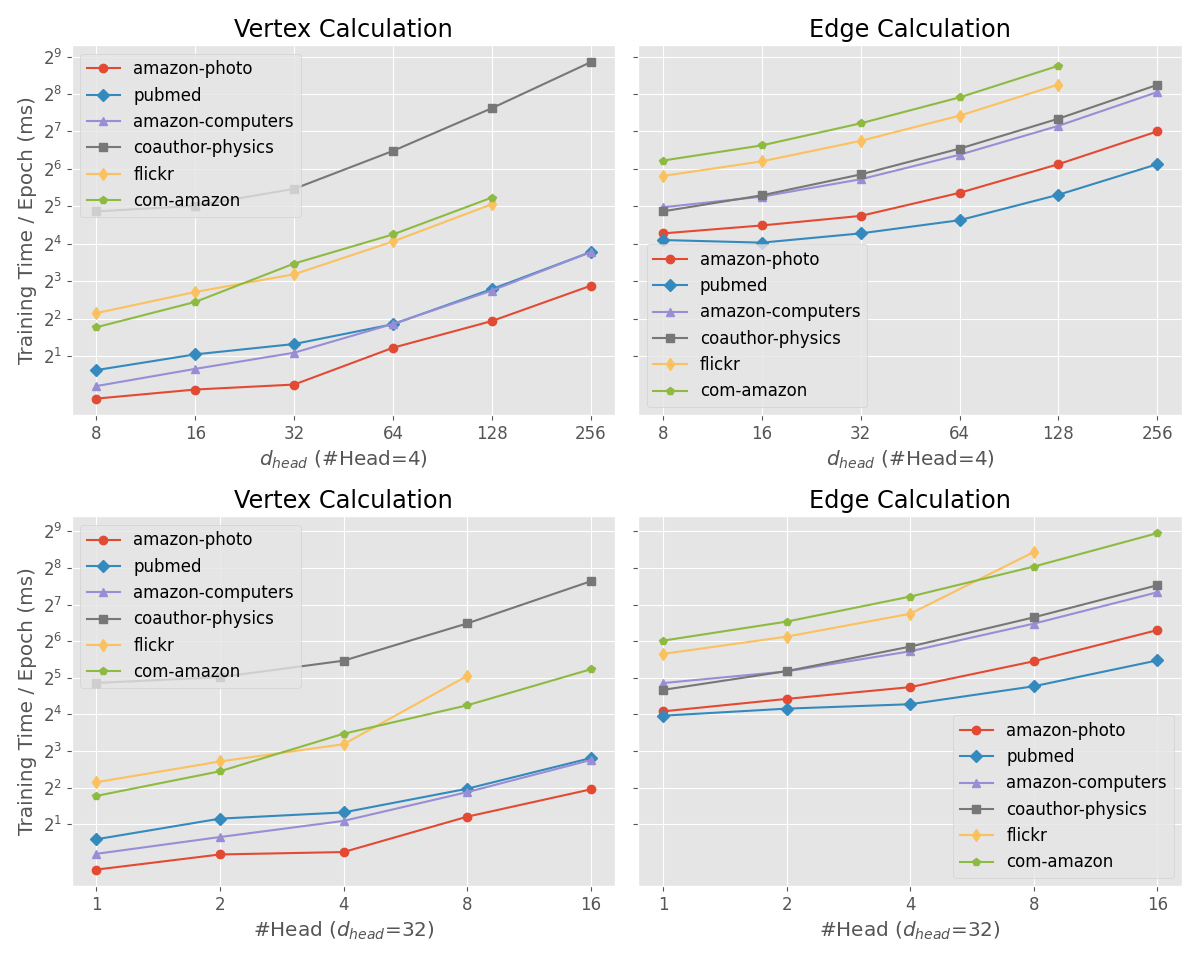
\includegraphics[height=8cm]{figs/experiments/exp_hyperparameter_on_vertex_edge_phase_time_gat.png}
    \caption{The influence of hyperparameters on GAT vertex/edge calculation time}
    \label{fig:exp_hyperparameter_on_vertex_edge_phase_time_gat}
\end{figure}

\begin{figure}
    \centering
    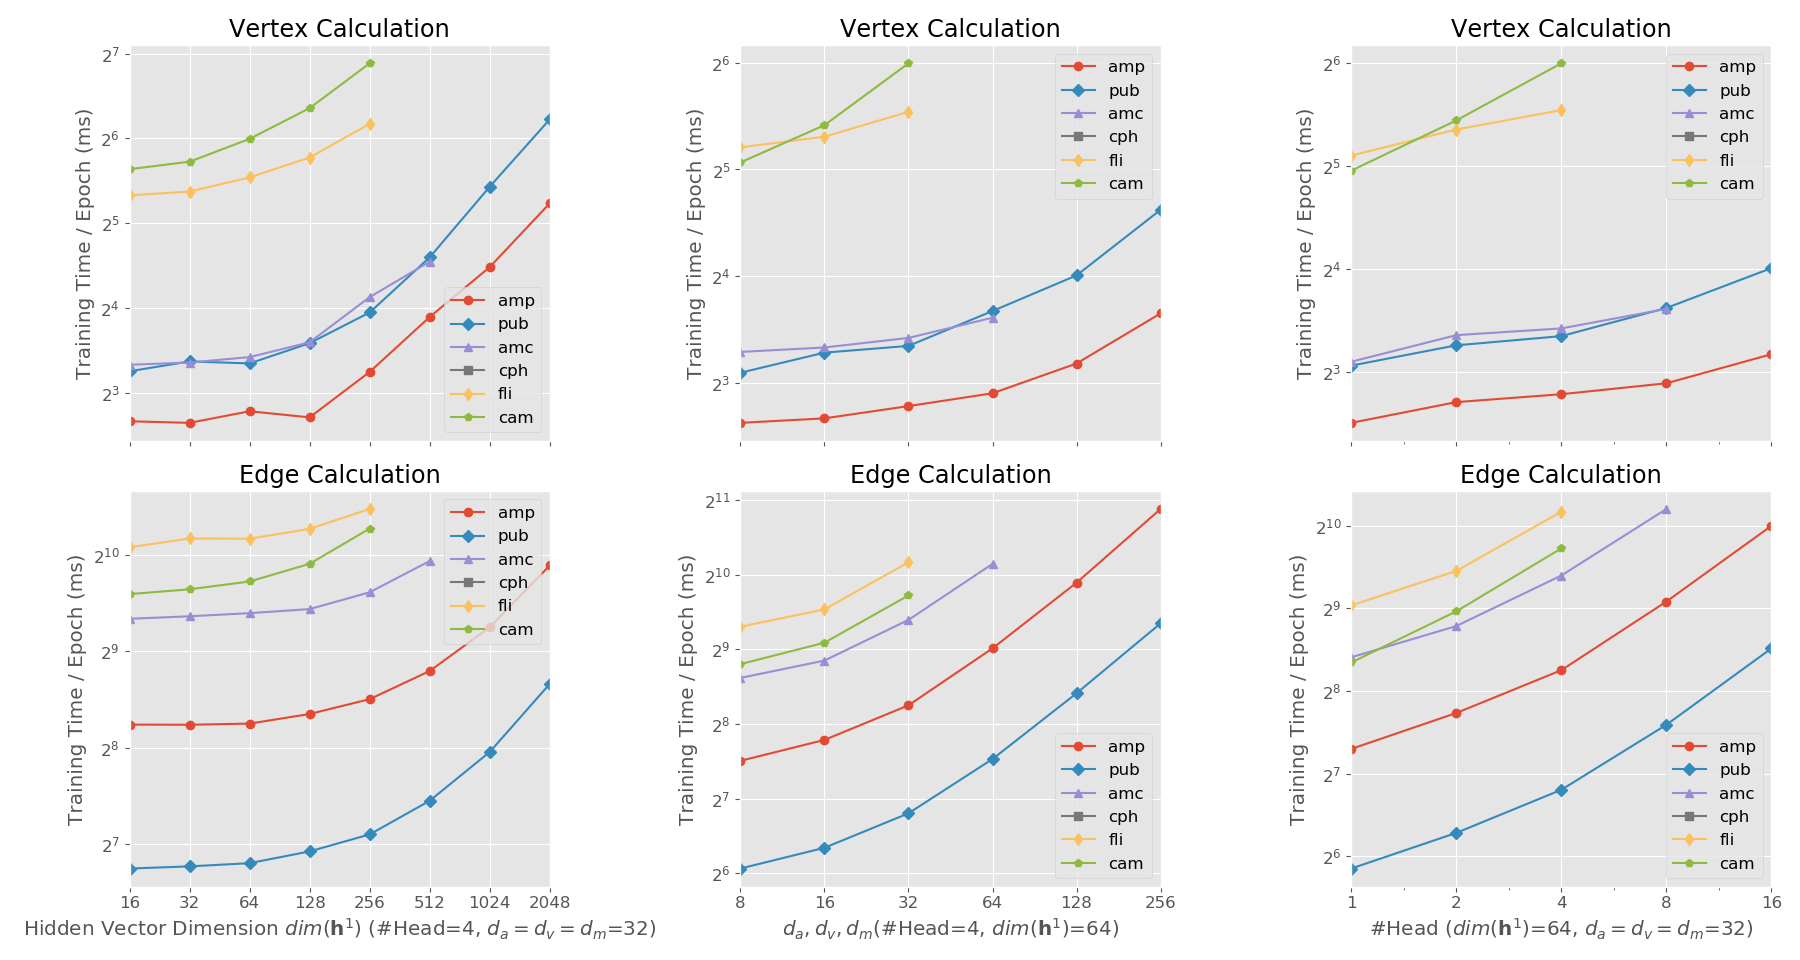
\includegraphics[height=8cm]{figs/experiments/exp_hyperparameter_on_vertex_edge_phase_time_gaan.png}
    \caption{The influence of hyperparameters on GaAN vertex/edge calculation time}
    \label{fig:exp_hyperparameter_on_vertex_edge_phase_time_gaan}
\end{figure}

\paragraph{The effects of hyper-parameters on memory usage}
\figurename~\ref{fig:exp_hyperparameter_memory_usage} shows how each GNN model's memory usage varies with the algorithm's hyperparameters.
With the increase of hyperparameters, GNN's memory usage also increases linearly.

\begin{figure}
    \centering
    \subfloat[GCN]{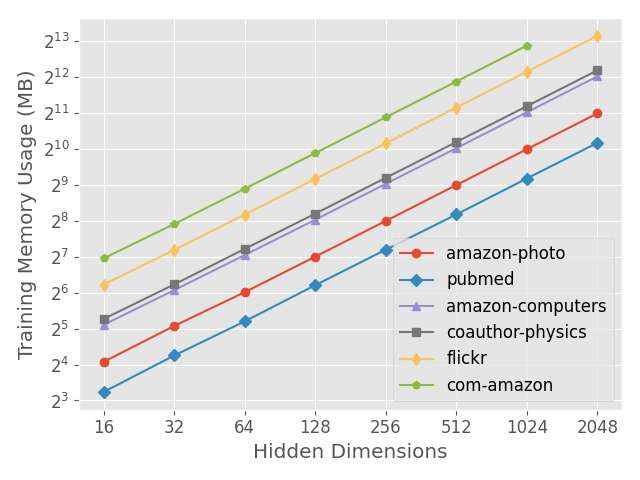
\includegraphics[height=4cm]{figs/experiments/exp_hyperparameter_on_memory_usage_gcn.png}}
    \subfloat[GGNN]{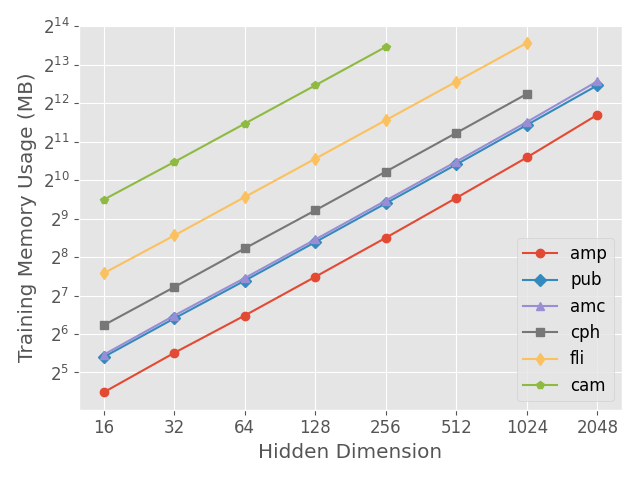
\includegraphics[height=4cm]{figs/experiments/exp_hyperparameter_on_memory_usage_ggnn.png}}\\
    \subfloat[GAT]{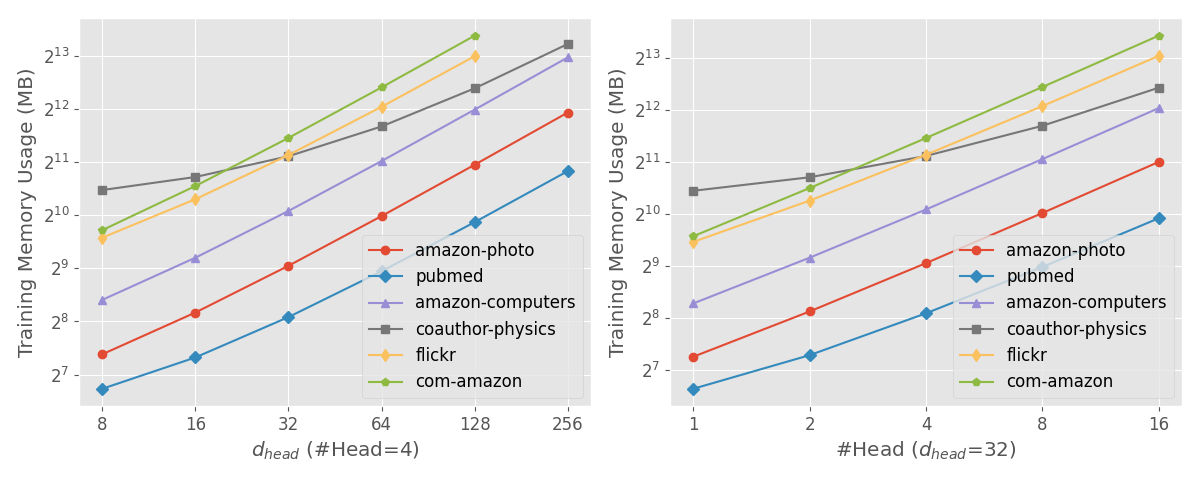
\includegraphics[height=4cm]{figs/experiments/exp_hyperparameter_on_memory_usage_gat.png}}\\
    \subfloat[GaAN]{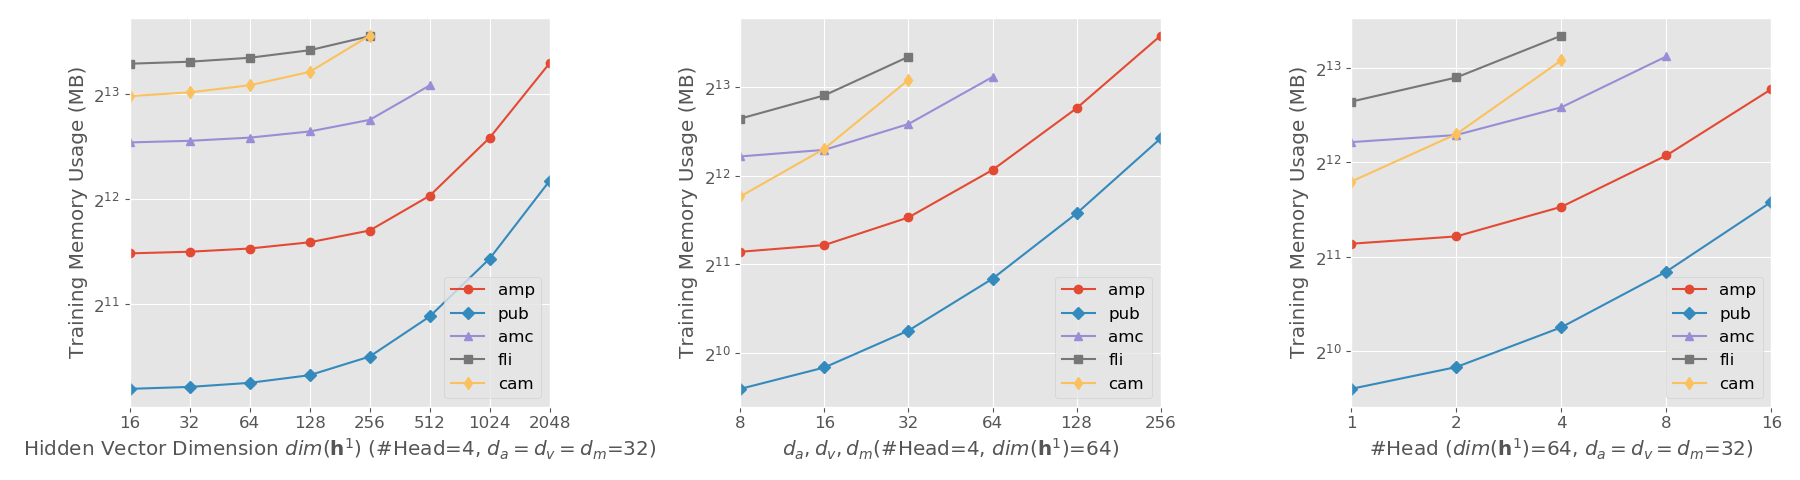
\includegraphics[height=4cm]{figs/experiments/exp_hyperparameter_on_memory_usage_gaan.png}}
    \caption{The effect of hyperparameters on GPU memory usage during the training phase (excluding the dataset memory)}
    \label{fig:exp_hyperparameter_memory_usage}
\end{figure}

\paragraph{Summary}

We can answer the question Q1 in \ref{sec:experimental_env}: the complexity analysis in \tablename~\ref{tab:gnn_overview_edge}, \tablename~\ref{tab:gnn_overview_vertex} is valid.
\textbf{GNN training time and memory usage are linearly related to hyperparameters}.
This allows algorithm engineers to use larger hyperparameters to increase the complexity of GNN without worrying about the time-consuming training and the explosive growth of memory usage.

\subsection{Training Time Breakdown}
\label{sec:training_time_breakdown}

In this subsection, we aims to find what stage is the most time-consuming stage in GNN training by decomposing the time-consuming training.

\paragraph{Vertex/edge calculation time-consuming proportion analysis}

\figurename~\ref{fig:exp_vertex_edge_cal_proportion} shows the ratio of the vertex/edge calculation time of different GNN layers
to the total training time (including forward, backward and evaluation). GCN spends most of time on edge calculation in most datasets. A special case is  \textit{cph} dataset because of
the dimension of the input feature vector of this dataset is very high, resulting in the high vertex calculation of Layer0.
High vertex calculation makes GGNN's vertex calculation time-consuming ratio significantly higher than other algorithms.
But in most datasets, for GGNN, edge calculation still occupies the majority of total time.
In \textit{pub} and cam dataset, the edge calculation cost and the vertex calculation cost are close for GGNN
because the average degree of the two datasets is low (only 4.5 and 2.8).
For the GAT and GaAN algorithms, due to their high edge calculation complexity, their edge calculation cost time is absolutely dominant.
In summary, \textbf{edge calculation is the main time-consuming factor of GNN training}, especially in the case of more complicated edge calculation.

Experiments also show that \textbf{the average degree of the dataset affects the time-consuming proportion of vertex/edge calculation}.
We use the R-MAT generator to generate random graphs with an average degree between 10 and 100. The number of nodes of these graphs is fixed at 50k.
Then we measure the change of the time-consuming proportion of the vertex/edge calculation in each GNN model varies with the average degree of the graph,
as shown in \figurename~\ref{fig:exp_avg_degree_on_vertex_edge_cal_time}. The edge calculation time increases linearly with the increase of the average degree,
\textbf{The edge calculation time dominates the entire calculation time in most cases}.
Only when the vertex calculation complexity is very high and the average degree is very low, the vertex calculation time can overtake the edge calculation time.
Therefore, \textbf{the focus of GNN training optimization should improve the efficiency of edge calculation}.

\begin{figure}
    \centering
    \subfloat[GCN]{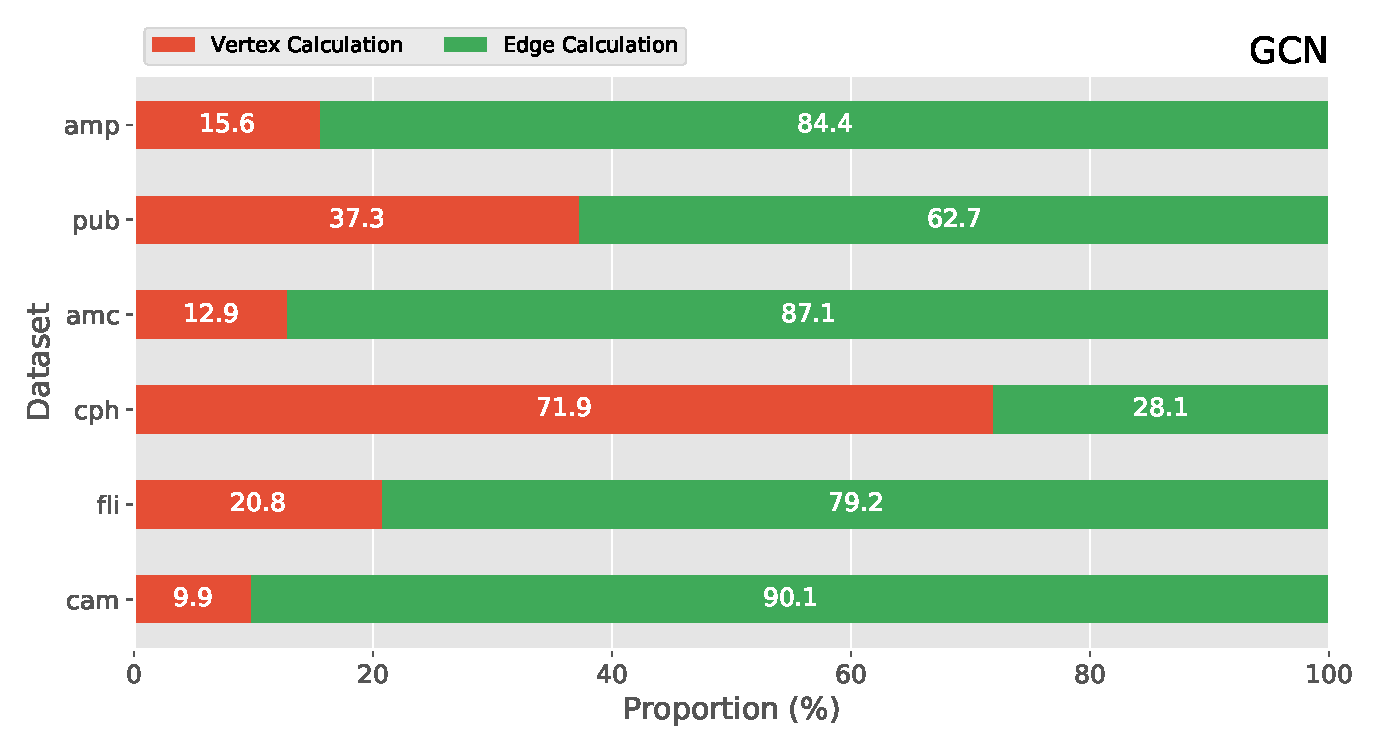
\includegraphics[height=4cm]{figs/experiments/exp_vertex_edge_cal_proportion_gcn.pdf}}
    \subfloat[GGNN]{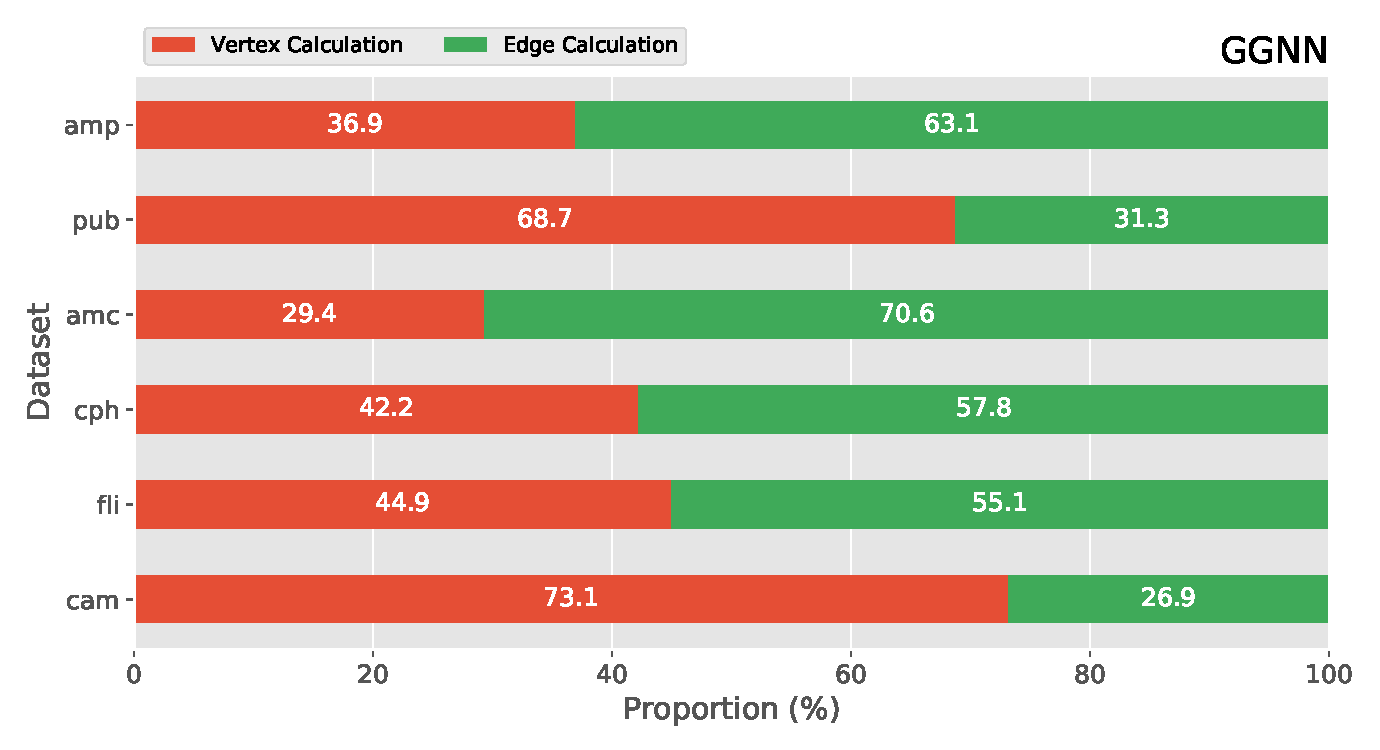
\includegraphics[height=4cm]{figs/experiments/exp_vertex_edge_cal_proportion_ggnn.pdf}}\\
    \subfloat[GAT]{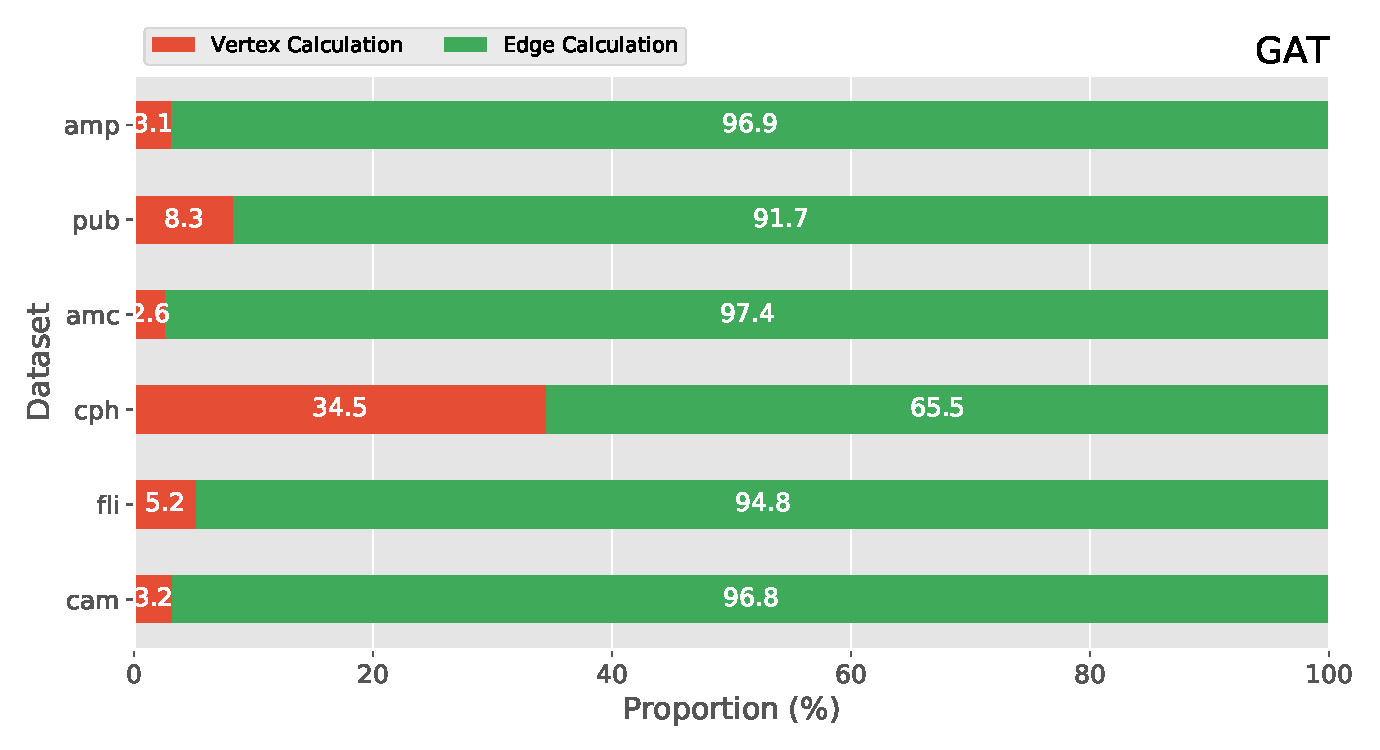
\includegraphics[height=4cm]{figs/experiments/exp_vertex_edge_cal_proportion_gat.pdf}}
    \subfloat[GaAN]{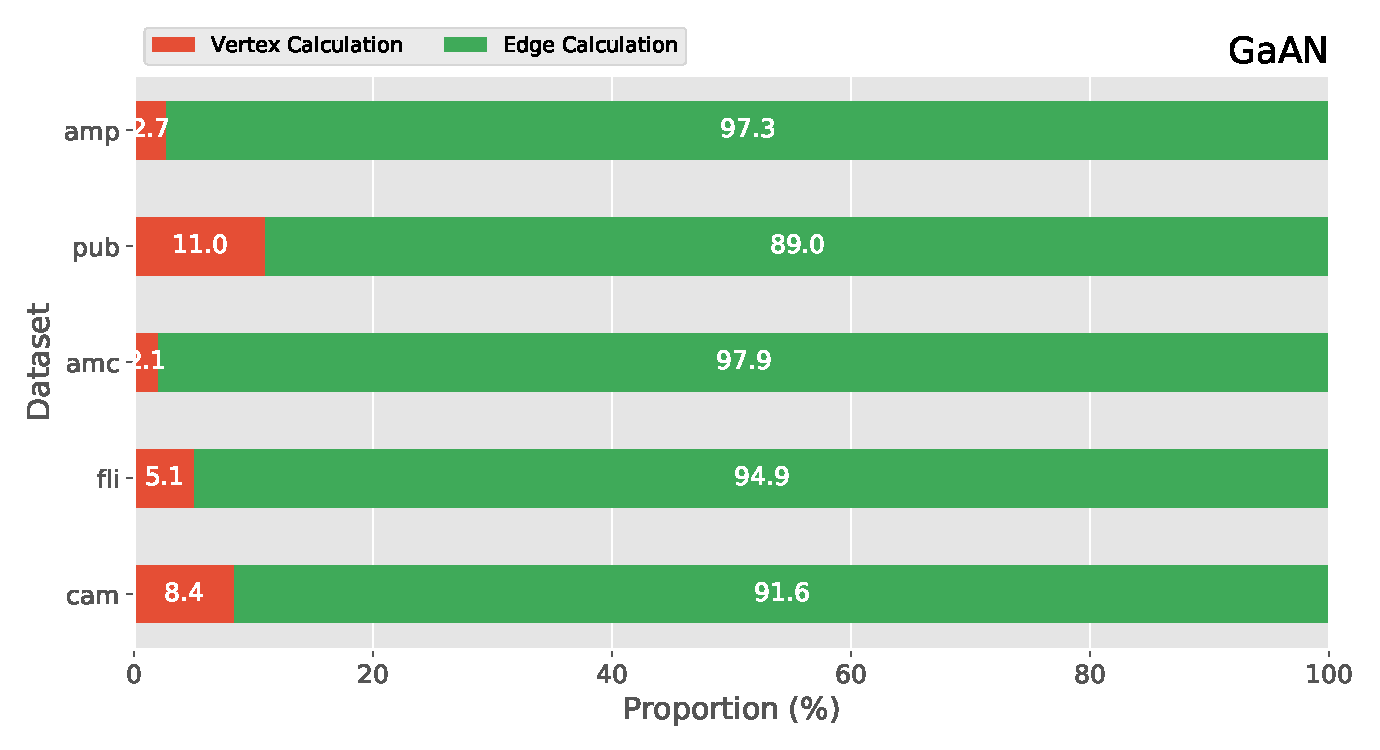
\includegraphics[height=4cm]{figs/experiments/exp_vertex_edge_cal_proportion_gaan.pdf}}
    \caption{Vertex/edge calculation time-consuming ratio.}
    \label{fig:exp_vertex_edge_cal_proportion}
\end{figure}

\begin{figure}
    \centering
    \subfloat[GCN]{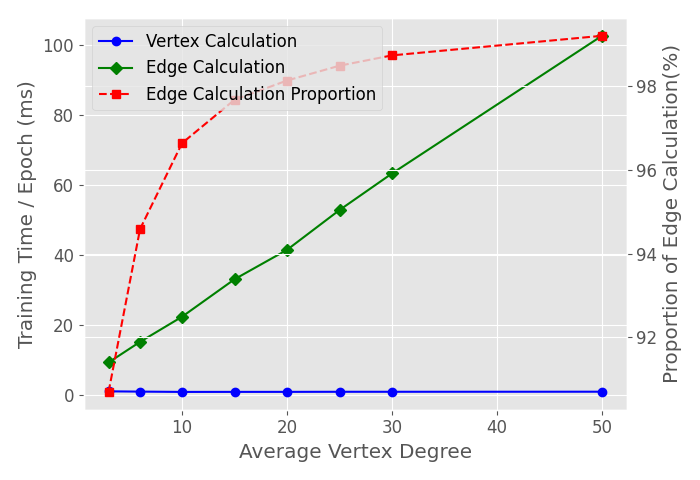
\includegraphics[height=4cm]{figs/experiments/exp_avg_degree_on_vertex_edge_cal_time_gcn.png}}
    \subfloat[GGNN]{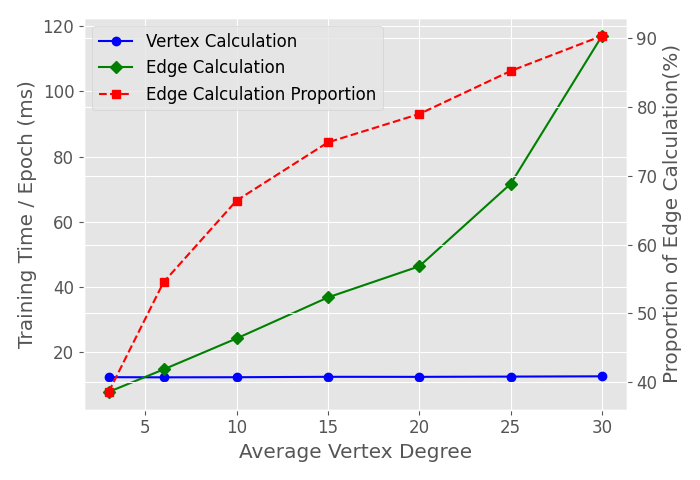
\includegraphics[height=4cm]{figs/experiments/exp_avg_degree_on_vertex_edge_cal_time_ggnn.png}}\\
    \subfloat[GAT]{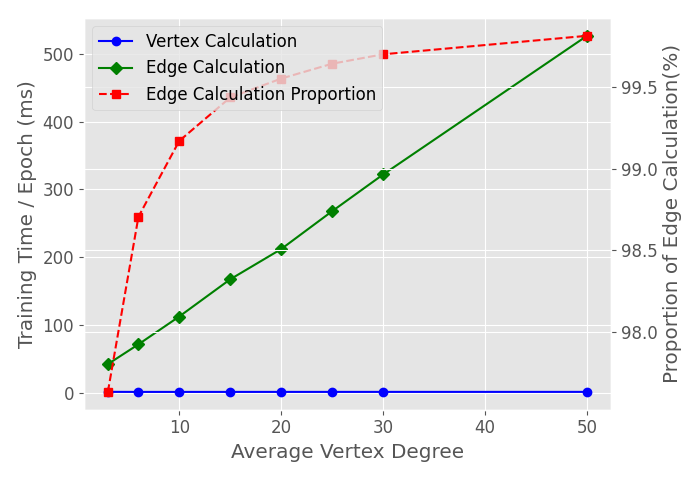
\includegraphics[height=4cm]{figs/experiments/exp_avg_degree_on_vertex_edge_cal_time_gat.png}}
    \subfloat[GaAN]{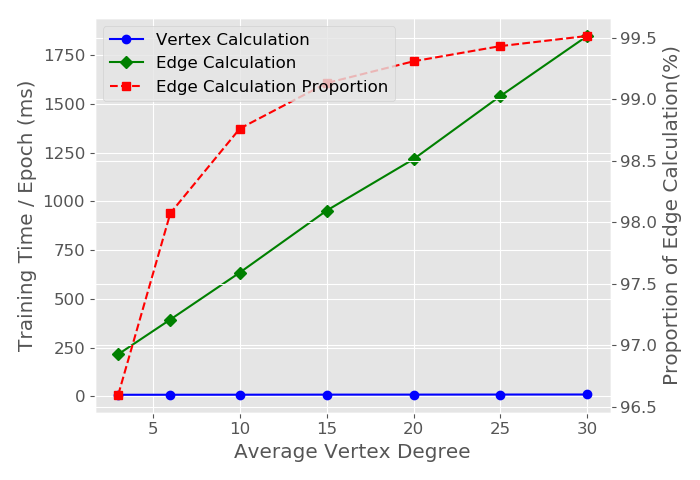
\includegraphics[height=4cm]{figs/experiments/exp_avg_degree_on_vertex_edge_cal_time_gaan.png}}
    \caption{The effect of the average vertex degree on the time-consuming proportion of vertex/edge calculation.}
    \label{fig:exp_avg_degree_on_vertex_edge_cal_time}
\end{figure}

\paragraph{Time-consuming decomposition analysis of edge calculation}

\begin{figure}
    \centering
    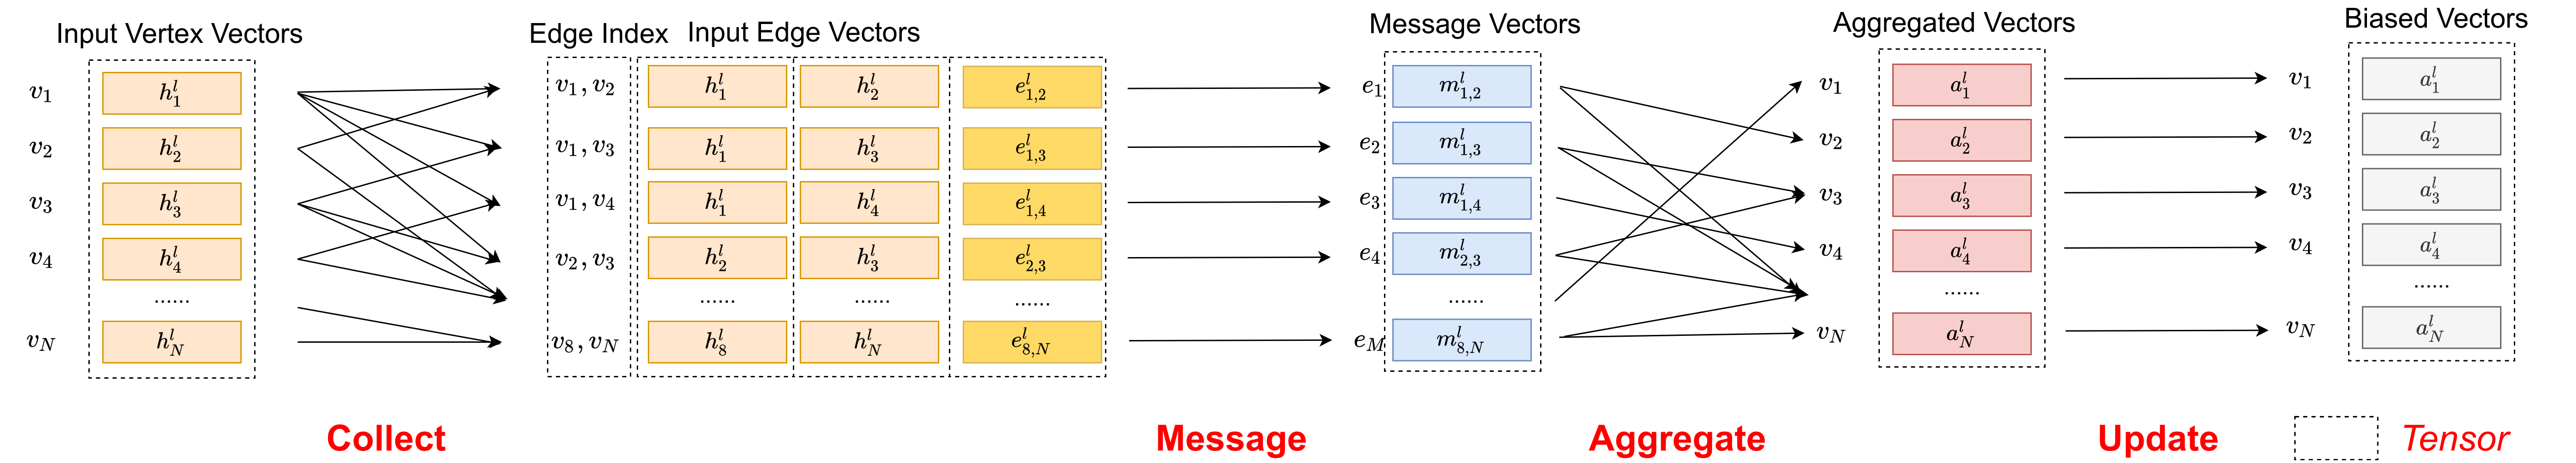
\includegraphics[width=1\columnwidth]{figs/illustration/steps_in_edge_calculation.png}
    \caption{Step decomposition of edge calculation}
    \label{fig:steps_in_edge_calculation}
\end{figure}

The edge calculation phase can be further decomposed into four steps of collect, message, aggregate and update,
as shown in \figurename~\ref{fig:steps_in_edge_calculation}. The figure shows the edge calculation process of GNN layer $l$,
edge index is a matrix that holds the edge sets of the graph with shape $M*2$, where $M$ is the number of edges,
and two columns of the matrix respectively store the source vertex and the target vertex of each edge.
Edge index remains unchanged throughout the calculation process.
The collect step is used to prepare data structure required for edge calculation and will use the vertex hidden vector of the GNN layer $\boldsymbol{h}_i^l (1 \leq i \leq N)$
as input, which is copied to the two layers of each edge according to the edge index, forming the input parameter tensor of the edge calculation function $\phi$
(including $\boldsymbol{h}_i^l$,$\boldsymbol{h}_j^ l$ and $\boldsymbol{e}_{j, i}^l$).
There is no calculation in this step, only data access is involved.
The message step calls the function given by the user $\phi$ to complete the edge calculation process, and get message vector of each edge $\boldsymbol{m}_{j, i}^l (\boldsymbol{e}_{j, i}^l \in E(G))$.
The aggregate step is based on the target of each edge, the message vector with the same target vertex is aggregated by the aggregation operator $\Sigma$,
and then each vertex aggregation vector $\boldsymbol{a}_i^l (1 \leq i \leq N)$ is obtained.
The last update step is optional, and it can perform additional correction processing on the aggregated vector (for example, adding bias to GCN).
The aggregated vector $a_i^l$ after the update process will be input into the vertex calculation function $\gamma$ as an input parameter.

We performed the execution time decomposition of the edge calculation process of each GNN algorithm on different datasets,
and the results are shown in \figurename~\ref{fig:exp_edge_calc_decomposition}.
The time-consuming decomposition of the edge calculation of each GNN is relatively stable and rarely affected by dataset.
Although the collect step only performs data preparation, it occupies a lot of execution time in all GNNs.
The message step in the GNN (GAT and GaAN) with high edge calculation complexity occupies the absolute dominant.
Although its edge calculation in GCN only has a simple multiplication operation, it still takes more than 20\% of the time;
In GGNN, because its edge calculation function $\boldsymbol{m}_{j,i }^l=\boldsymbol{W}^l\boldsymbol{h}_{j}^l$ is only related to the source vertex,
so in the implementation of PyG will be $\boldsymbol{W}^l\boldsymbol{h}_j The calculation of ^l$ is carried out before the edge calculation starts
(because this part of the calculation is only related to vertices, so we count the calculation into the vertex calculation phase).
The calculated result is cached, and it is directly read when the message step is performed. As a result, the message step of GGNN gets 0.
For the aggregate step, it occupies at least 35\% of training time of GNN (GCN and GGNN) with low edge computational complexity,
while the GNN with high edge computational complexity (GAT and GaAN), whose time consumption is close to the collect step,
and both are much lower than the message step. Experiments show that \textbf{for an algorithm with high edge calculation complexity,
    the message step is the bottleneck of its performance, and it should be optimized}; and \textbf{For algorithms with low computational complexity,
    optimizing the collect and aggregate steps can significantly reduce training time}.

\begin{figure}
    \centering
    \subfloat[GCN]{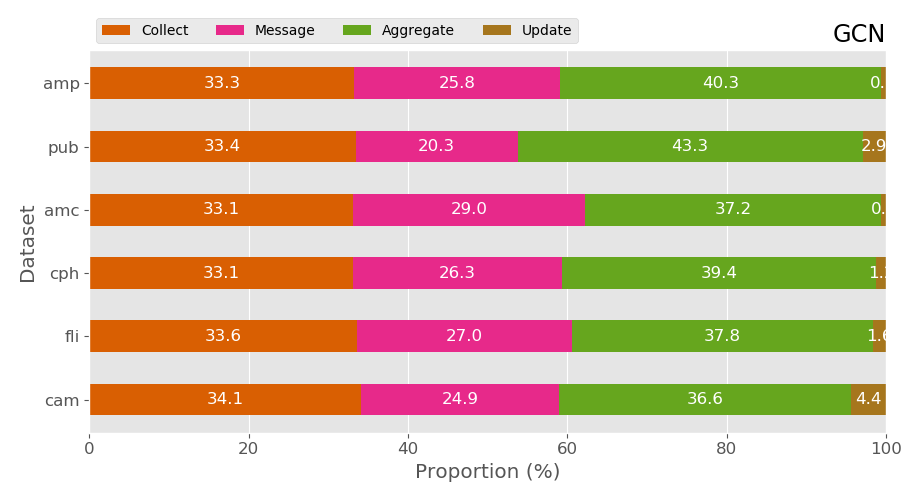
\includegraphics[height=4cm]{figs/experiments/exp_edge_calc_decomposition_gcn.png}}
    \subfloat[GGNN]{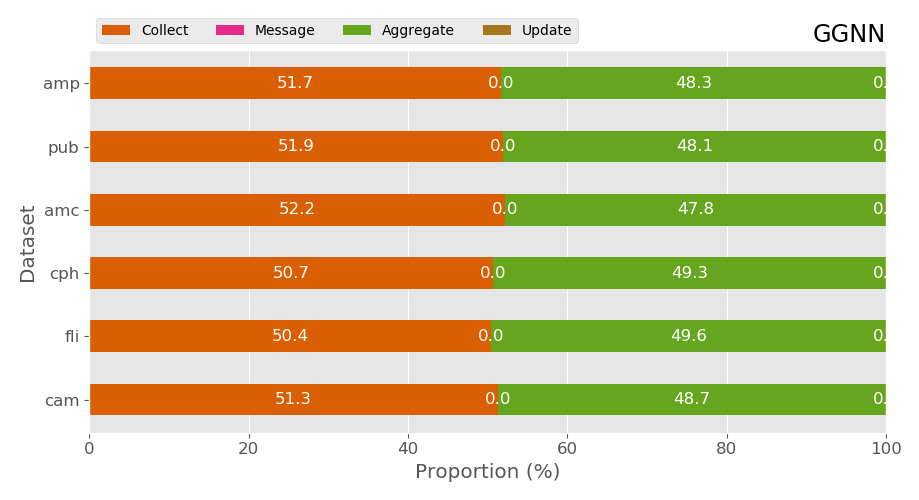
\includegraphics[height=4cm]{figs/experiments/exp_edge_calc_decomposition_ggnn.png}}\\
    \subfloat[GAT]{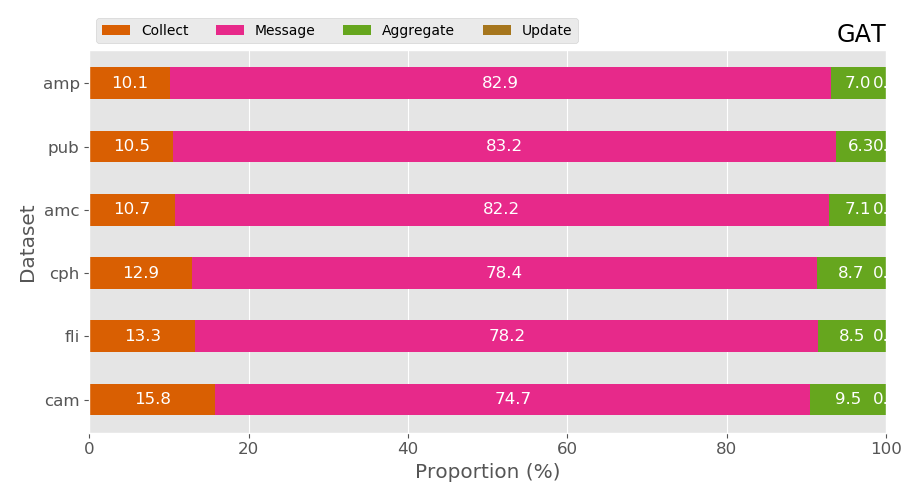
\includegraphics[height=4cm]{figs/experiments/exp_edge_calc_decomposition_gat.png}}
    \subfloat[GaAN]{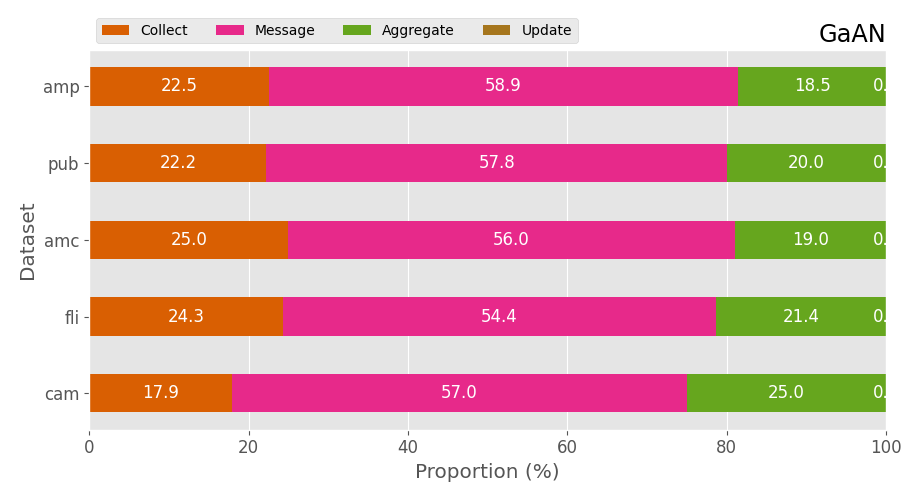
\includegraphics[height=4cm]{figs/experiments/exp_edge_calc_decomposition_gaan.png}}
    \caption{Time-consuming decomposition of edge calculations (including Layer0 and Layer1).}
    \label{fig:exp_edge_calc_decomposition}
\end{figure}

\paragraph{Hot-spot operator analysis}
Various functions for vertex/edge calculation $\phi, \Sigma,\gamma$ consist of a series of basic operators,
which are mapped to specific basic operators on the GPU (matrix multiplication mm, elementwise multiplication mul and index by tensor index\_select)

Figure~\ref{fig:exp_top_basic_ops} shows the five operators with the highest time-consuming proportion in each GNN,
the operator in the legend The order is determined by the average time-consuming ratio.

\begin{figure}
    \centering
    \subfloat[GCN]{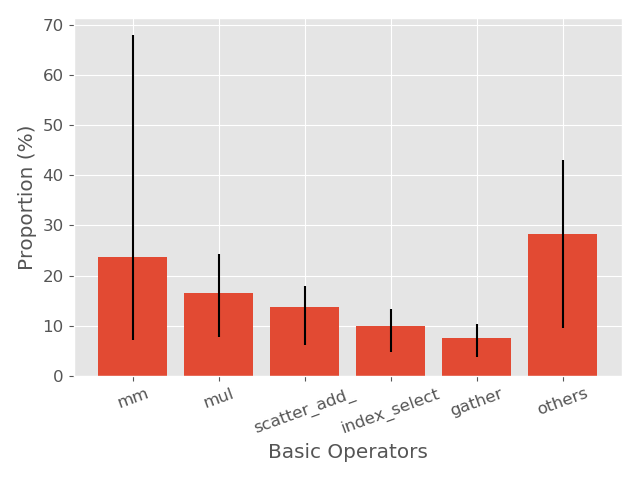
\includegraphics[height=4cm]{figs/experiments/exp_top_basic_ops_gcn.png}}
    \subfloat[GGNN]{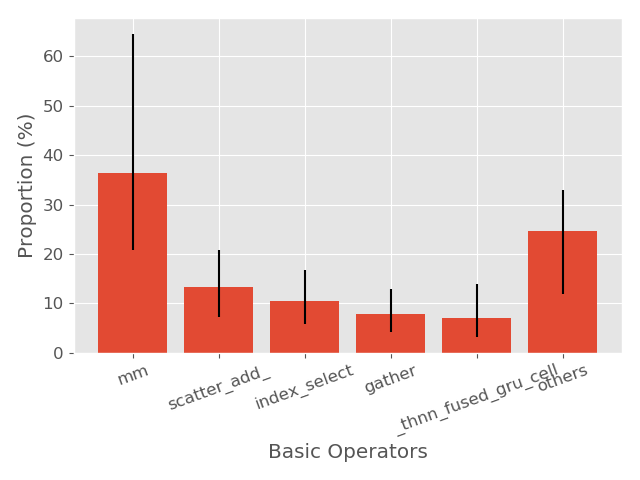
\includegraphics[height=4cm]{figs/experiments/exp_top_basic_ops_ggnn.png}}\\
    \subfloat[GAT]{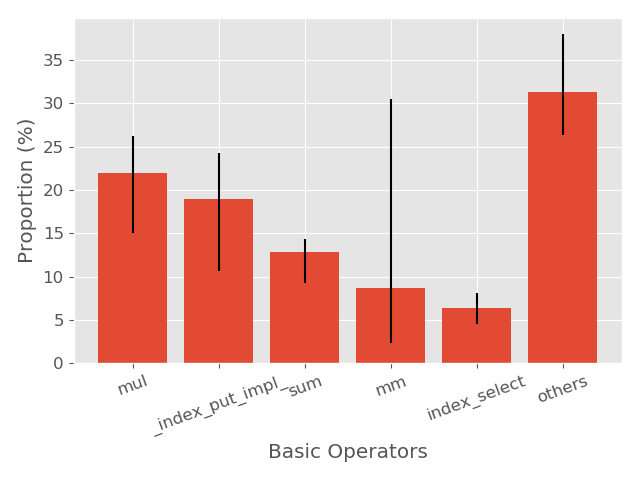
\includegraphics[height=4cm]{figs/experiments/exp_top_basic_ops_gat.png}}
    \subfloat[GaAN]{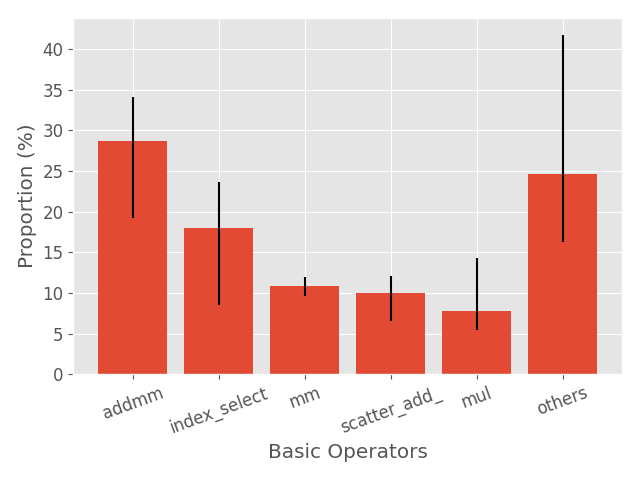
\includegraphics[height=4cm]{figs/experiments/exp_top_basic_ops_gaan.png}}
    \caption{The time-consuming ratio of basic operators (including the forward, backward and evaluation stages)}
    \label{fig:exp_top_basic_ops}
\end{figure}

The analysis of the time-consuming operators of each algorithm is as follows:

\begin{enumerate}
    \item The matrix multiplication operator mm in GCN is mainly used for vertex calculation $\gamma$,
          this operator is particularly time-consuming on the \textit{cph} dataset,
          because the dimensionality of the vertex feature vector input by \textit{cph} is very high,
          making the matrix multiplication in the vertex calculation of Layer0 The calculation is very high.
          Mul is the multiplication operation in the edge calculation function $\phi$.
          Both scatter\_add and gather are used to implement the aggregation step $\Sigma$ in the edge calculation,
          where the former is used in the forward stage and the latter is used in backward Phase.
          The index\_select operator is used in the collect step of the edge calculation.
          For the GCN algorithm, the edge calculation related operators occupy the main time-consuming.
          The time-consuming among the operators is relatively average, and there is no particularly outstanding performance bottleneck.
    \item The most time consuming in GGNN is also the matrix multiplication mm operator,
          which is mainly used for the vertex calculation function $\gamma$. The scatter\_add, index\_select and gather operators
          are used for edge calculations. And the \_thnn\_fused\_gru\_cell is used in the backward calculation of GRU.
          GGNN because of vertices With the increase in calculation complexity, the time-consuming time of the mm operator has increased significantly.
    \item The four most time-consuming operators in GAT are all related to the edge calculation.
          Mul, \_index\_put\_impl and sum are used to implement the edge calculation function $\phi$.
          The index\_select operator is used in the collect phase of the edge calculation.
          The mm operator is used vertex calculation function $\gamma$.
    \item The most time-consuming matrix multiplication operator mm in GaAN is used for both edge calculation and vertex calculation,
          where edge calculation is dominant. Mul and cat are used for the $\phi$ function in edge calculation.
\end{enumerate}

In terms of commonality,
\textbf{The main time-consuming of GNN calculation is still matrix multiplication mm, elementwise multiplication mul},
so it is very suitable for calculation with GPU. Although the calculation of the aggregate step in edge calculation is relatively simple,
but it involves data synchronization and non-regular calculations (the degree of different vertices is very different),
the related operators scatter\_add and gather still occupy a certain amount of time.
Although the collection step in the edge calculation does not have any calculationss,
but the related calculations index\_select operator still accounts for about 10\% of the time-consuming.
\textbf{aggregate step and collect step are one of the computational performance bottlenecks of all GNN training},
optimizing the corresponding operator will improve the training efficiency of all GNNs.

\paragraph{Summary of performance bottlenecks}

\begin{itemize}
    \item \textbf{The performance bottleneck of GNN training is affected by the average degree of the dataset}.
          Because the average degree of most real-world graphs is above 10 degrees \cite{network-repository},
          the performance bottleneck of GNN training will be concentrated on the edges calculation section.
    \item \textbf{According to the calculation complexity of the edge calculation function $\phi$, the performance bottleneck of GNN in edge calculation is different}:
          \begin{itemize}
              \item If the computational complexity of $\phi$ is high, the performance bottleneck is concentrated on the basic operators used to implement $\phi$.
                    Optimizing the implementation of the corresponding basic operators will improve the training performance of this type of GNN.
                    Taking GAT as an example, The most time-consuming operator \_index\_put\_impl in GAT is mainly used in the backward stage of the softmax calculation ($\alpha^k_{ij}$) in $\phi$,
                    which only involves data movement.
                    The optimized softmax implementation on the GPU can significantly reduce GAT training time.
              \item If the computational complexity of $\phi$ is low, the collect and aggregate steps in its edge calculation are bottlenecks in computational performance. The collect step only involves a large amount of data movement. The aggregate step calculation is relatively simple (such as sum/average/maximum) Value, etc.), but because it involves data synchronization and irregular calculation, its time-consuming is still significant.
                    Optimizing the implementation of these two steps on the GPU will improve the training performance of this type of GNN.
          \end{itemize}
\end{itemize}


\subsection{Memory Usage Analysis}

At present, all data (including datasets and intermediate calculation results) of PyG in the process of training GNN with GPU
are stored in GPU memory. Compared with the main memory of the system, the memory capacity on GPU is very limited.
\textbf{GPU memory capacity is limited to Determinants of the size of the training dataset}.
GaAN was unable to complete the training due to memory overflow during the training of the `\textit{cph}` dataset.

\begin{figure}
    \centering
    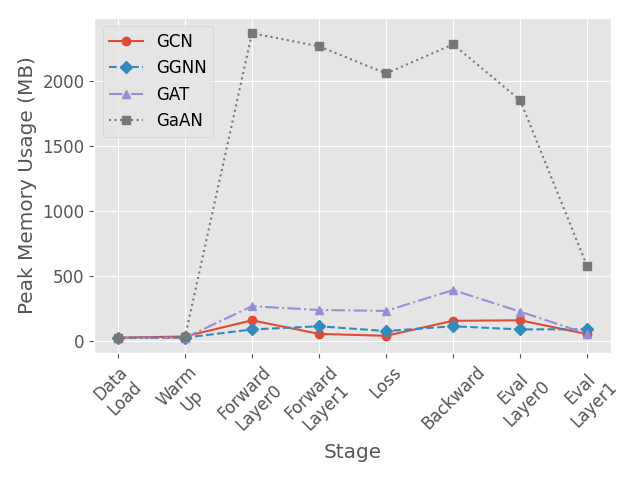
\includegraphics[width=0.7\columnwidth]{figs/experiments/exp_memory_usage_stage_amp.png}
    \caption{Maximum memory usage in each stage. Data Load refers to memory usage after data is loaded. dataset: amp. Other datasets are similar}
    \label{fig:exp_memory_usage_stage_amp}
\end{figure}

\figurename~\ref{fig:exp_memory_usage_stage_amp} shows the peak memory usage of each stage when each GNN is trained on the cam dataset, the situation is similar on other datasets.
\textbf{The memory usage in GNN training is forward The peak in the phase and the backward phase},
because a large number of temporary calculation results will be generated in the forward phase,
and the key intermediate calculation results will be cached.
The cached intermediate results will be used in the gradient calculation of the backward phase.
\figurename~\ref{fig:ggnn_vertex_func_computation_graph} shows the calculation graph of GGNN's vertex calculation function $\gamma$.
It can be seen that a large number of operators are involved in GGNN vertex calculation and a large number of intermediate calculation results are generated.The key calculation results will also be cached,
which is exacerbated Memory usage. Most of the peak memory usage in the loss phase comes from the intermediate calculation results of the cache.
With the end of the backward phase, the memory of the intermediate calculation results is released.
In the evaluation phase, there is no need to cache intermediate results for gradient calculations, Peak memory usage dropped significantly.

\begin{figure}
    \centering
    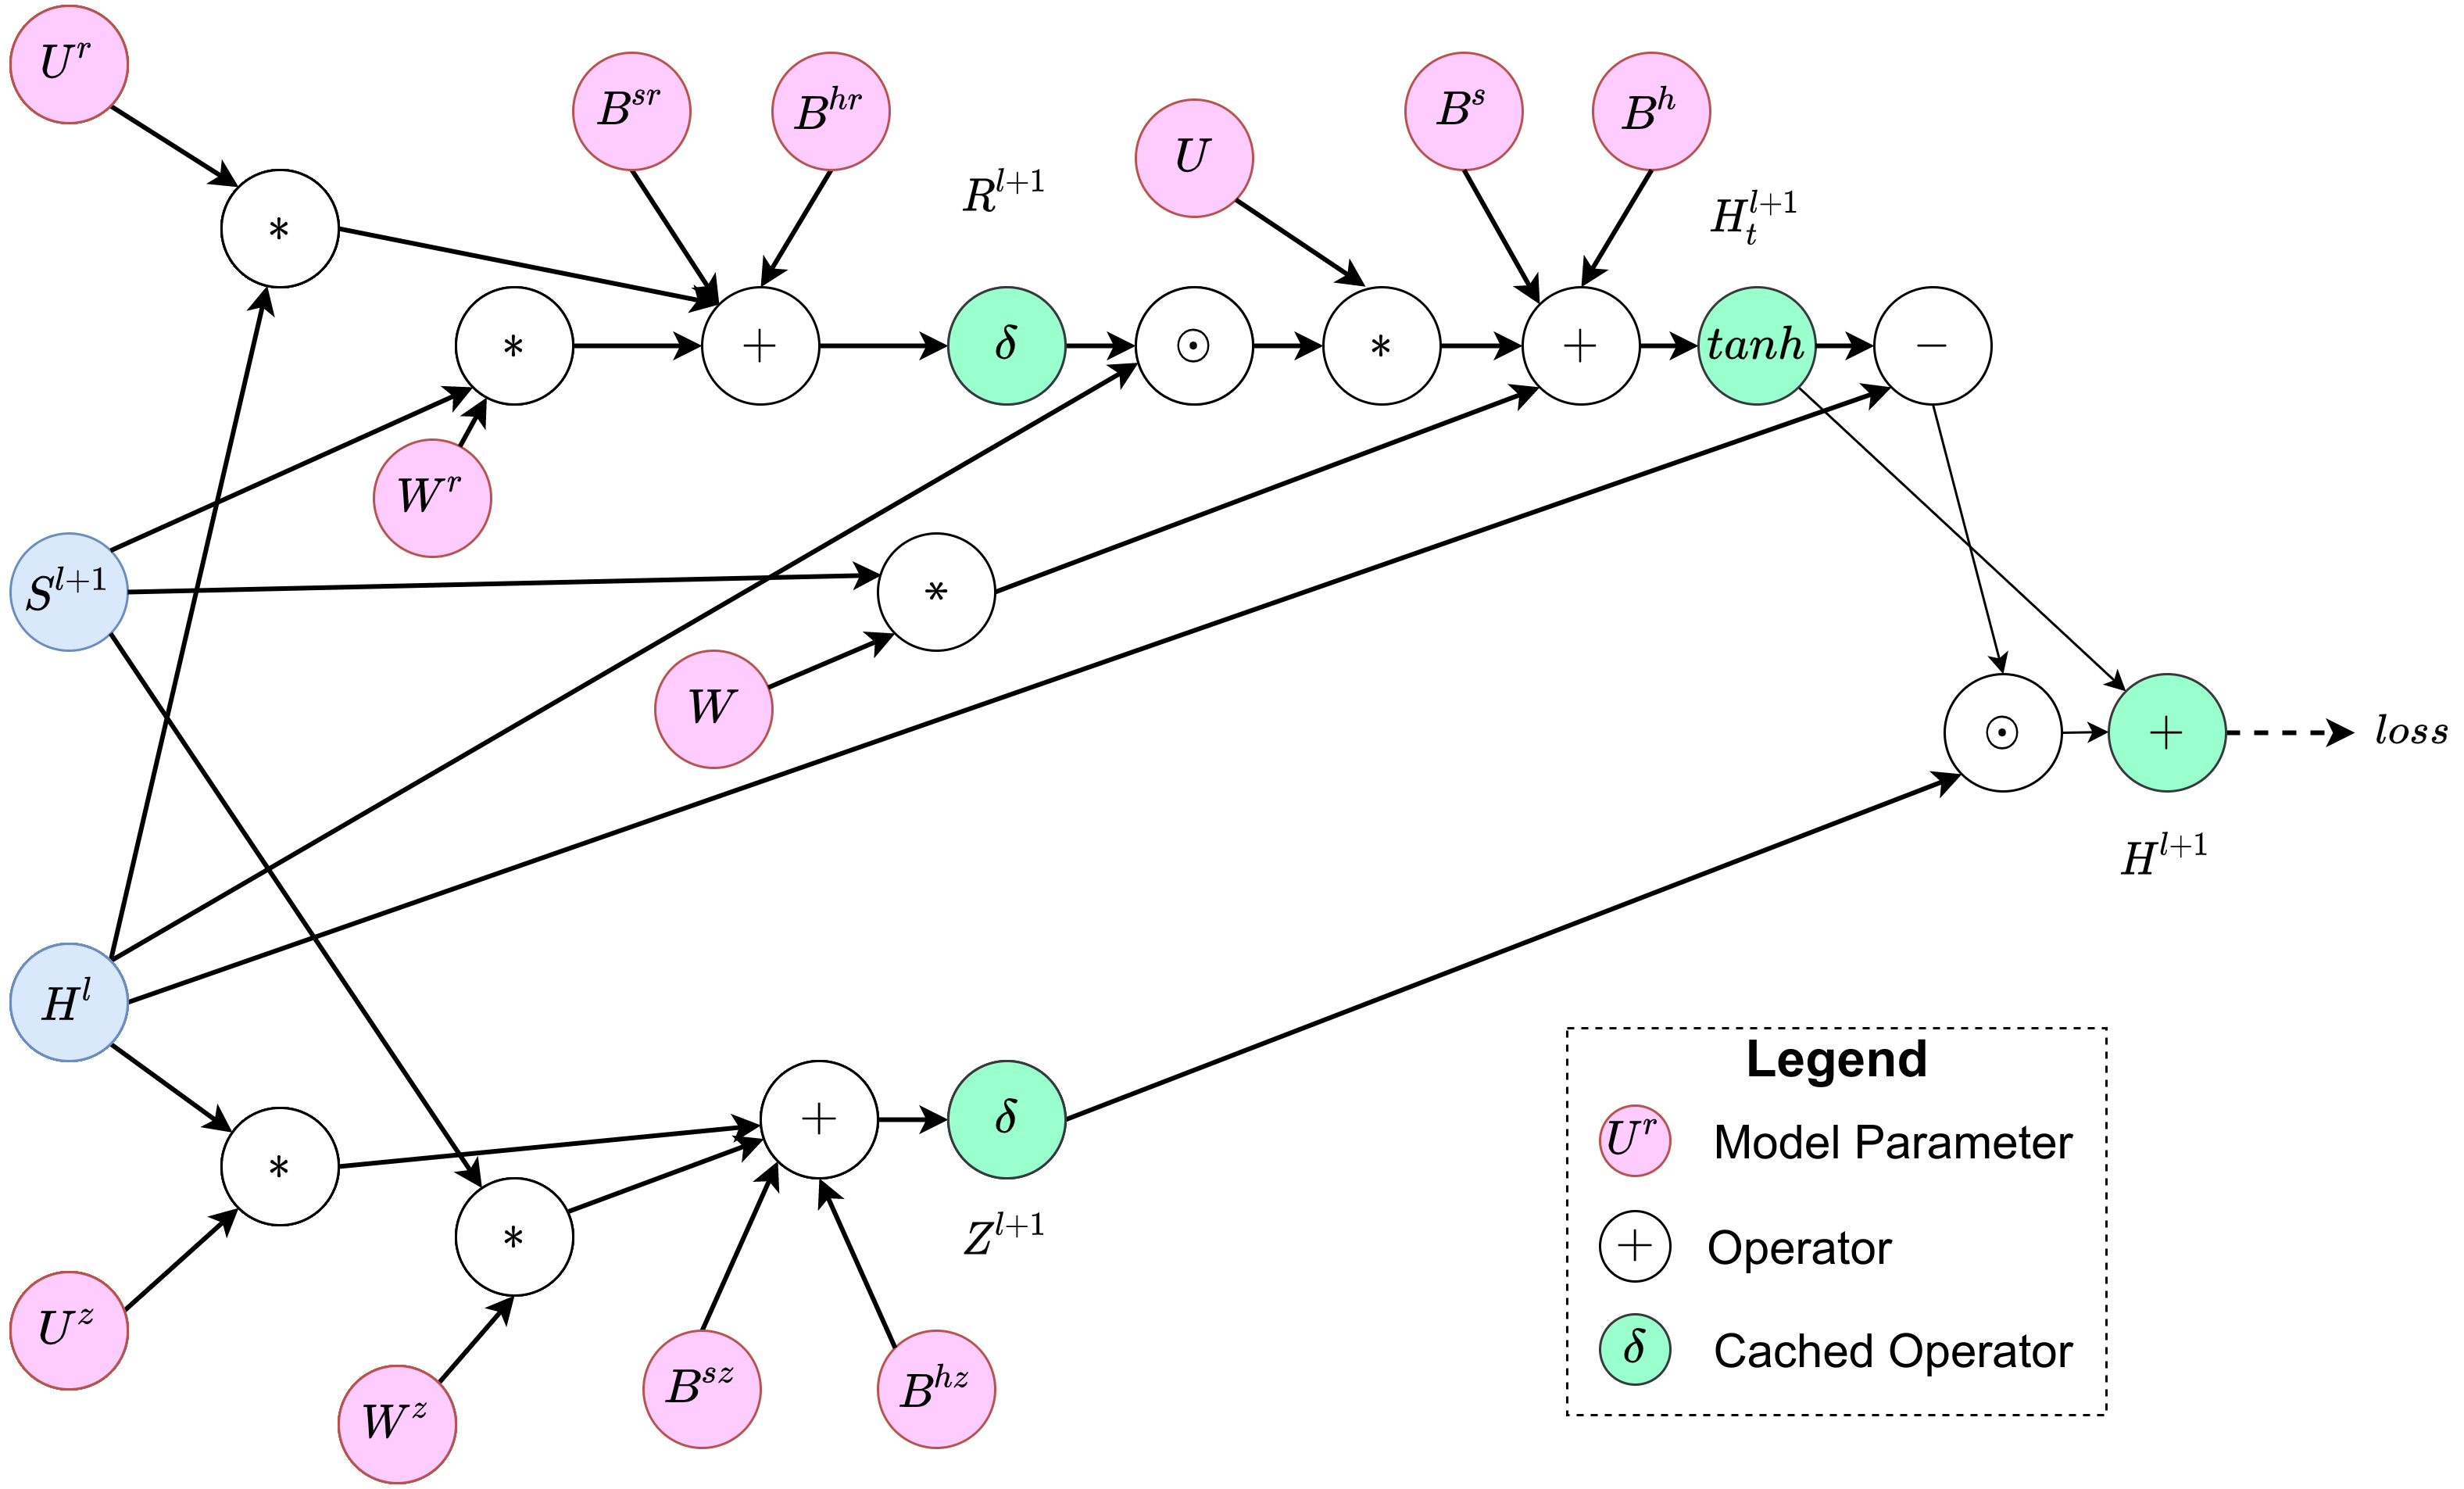
\includegraphics[width=0.7\columnwidth]{figs/illustration/ggnn_vertex_func_computation_graph.png}
    \caption{The calculation graph of the GGNN vertex calculation function $\gamma$. The output of the Cached Operator will be cached for gradient calculation in the backward process}
    \label{fig:ggnn_vertex_func_computation_graph}
\end{figure}

It is worth noting that \textbf{the peak memory during GNN training far exceeds the memory usage of the dataset itself}.
The ratio of the highest peak memory usage during our training compared to the memory usage after data Load is
defined as the memory expansion ratio. \figurename~\ref{fig:exp_memory_expansion_ratio} compares the memory expansion ratios
of different GNNs on different datasets. The expansion ratio of GCN is the lowest, between 5-14 times,
and the expansion ratio of GaAN is the highest, up to 101 times.
\textbf{Very high expansion ratio severely limits the data scalability of GNN, making GPU unable to process large-scale graph datasets},
especially restricting GNN with high edge calculation complexity.

\begin{figure}
    \centering
    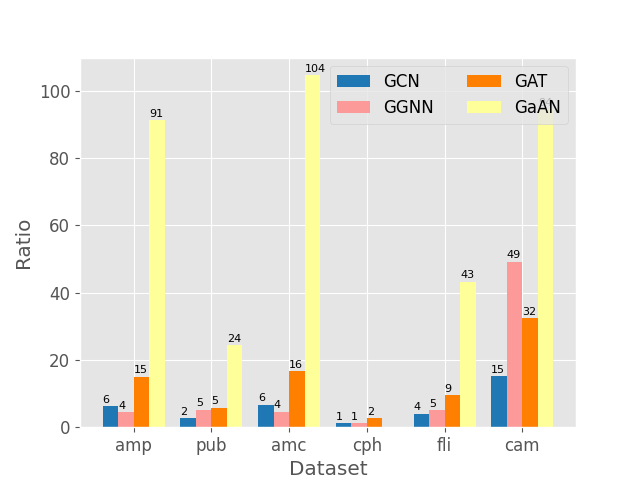
\includegraphics[width=0.7\columnwidth]{figs/experiments/exp_memory_expansion_ratio.png}
    \caption{The proportion of memory expansion of each GNN on different datasets.}
    \label{fig:exp_memory_expansion_ratio}
\end{figure}

\figurename~\ref{fig:exp_memory_expansion_ratio} also shows that the expansion ratio of the same GNN under the same hyperparameters changes with different datasets.
Because the input feature dimension of the \textit{cph} dataset is much higher than the hidden vector of the GNN layer The dimension of the input feature vector matrix
of the graph is much higher than the matrix size of the intermediate calculation result of the cache,
so its expansion ratio is particularly low, and the cam dataset is the opposite. In order to measure the effect of the input feature vector dimension on the memory
expansion ratio , We randomly generated feature vectors of specific dimensions for different datasets.
\figurename~\ref{fig:exp_memory_expension_ratio_input_feature_dimension} shows the change in the expansion ratio under different input feature vector dimensions.
\textbf{In the same GNN structure and hyperparameter settings, using a higher-dimensional input feature vector can reduce memory expansion ratio} .

\begin{figure}
    \centering
    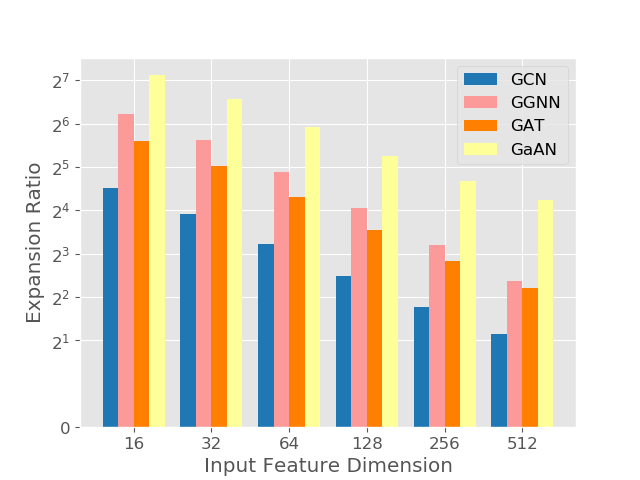
\includegraphics[width=0.7\columnwidth]{figs/experiments/exp_memory_expansion_ratio_input_feature_dimension_com-amazon.png}
    \caption{The change of the memory expansion ratio with the dimension of the input feature vector. dataset: cam, other datasets are similar}
    \label{fig:exp_memory_expension_ratio_input_feature_dimension}
\end{figure}

Different GNNs have different vertex/edge calculation complexity, and the scale of the generated intermediate results has different sensitivity
to the number of vertices/edges in the graph, resulting in the memory expansion ratio being affected by the average degree of the graph.
We measured the GPU peak memory The usage and expansion ratios are affected by the scale of the graph.

In the case of a fixed number of vertices in the graph, we use the R-MAT generator to generate random graphs with different average degrees (number of edges).
The \figurename~\ref{fig:exp_memory_expansion_ratio_input_graph_number_of_edges} shows how the memory usage during training varies with the average degree.
\textbf{As the average degree increases, the peak memory usage increases linearly.
    The intermediate results generated by the edge calculation gradually dominate, and the memory expansion ratio of each GNN gradually stabilizes}.
The expansion ratio is affected by the complexity of the edge calculation.
Except for GGNN, the memory expansion ratio of other GNNs increases with the increase of degree. GGNN has a high vertex calculation complexity.
When the average degree is low, its memory expansion ratio is mainly affected by the intermediate results of vertex calculation;
when the average When the degree is increased, the memory expansion ratio is gradually determined by the edge calculation complexity.
Because GGNN has the lowest edge calculation complexity, its stable expansion ratio is the lowest.

\begin{figure}
    \centering
    \subfloat[]{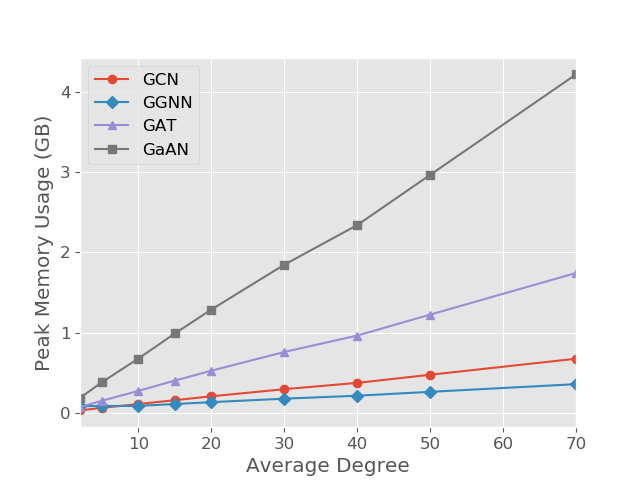
\includegraphics[height=4cm]{figs/experiments/exp_memory_expansion_ratio_input_graph_number_of_edges_peak_memory.png}}
    \subfloat[]{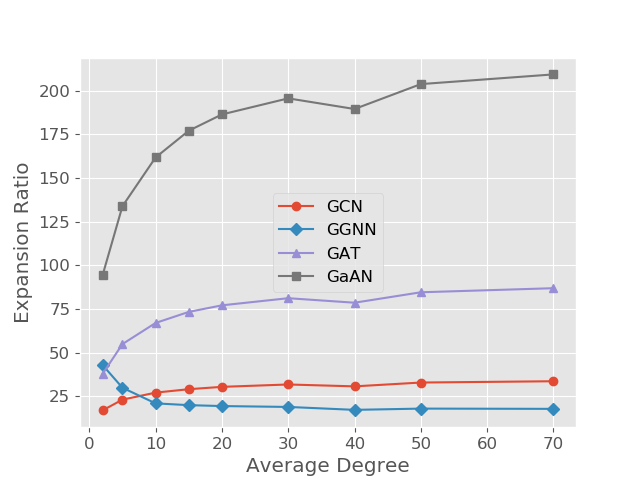
\includegraphics[height=4cm]{figs/experiments/exp_memory_expansion_ratio_input_graph_number_of_edges_expansion_ratio.png}}
    \caption{The change of memory usage with the average degree of the graph (R-MAT random graph, the number of vertices is fixed at 10k, and the input feature vector dimension is 32}
    \label{fig:exp_memory_expension_ratio_input_feature_dimension}
\end{figure}

In the case of a fixed number of edges in the graph, we use the R-MAT generator to generate random graphs with different numbers of vertices
\figurename~\ref{@fig:exp_memory_expansion_ratio_input_graph_number_of_vertices_fixed_edge} shows the change of memory usage with the number of vertices during training.
Except for GGNN, the number of vertices increases, the number of vertices increases, the number of vertices increases,
and the number of vertices increases. The size of the eigenvector matrix of the vertex input becomes larger,
but the peak memory usage only increases slightly, which makes the proportion of memory expansion decrease to a certain extent.
Only GGNN has a large number of intermediate calculation results during the vertex calculation process because of the high vertex calculation complexity.
The memory expansion factor has a small increase. The experimental data shows that \textbf{the intermediate result produced by the edge calculation is the dominant factor
    in memory usage, and the peak memory usage of each GNN increases linearly with the increase in the number of edges}.

\begin{figure}
    \centering
    \subfloat[]{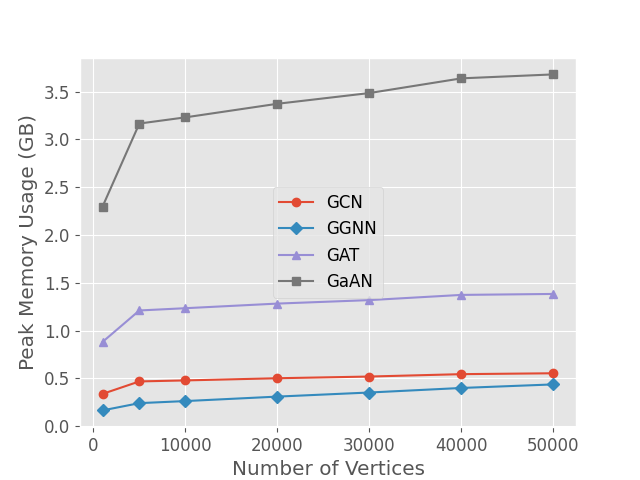
\includegraphics[height=4cm]{figs/experiments/exp_memory_expansion_ratio_input_graph_number_of_vertices_fixed_edge_peak_memory.png}}
    \subfloat[]{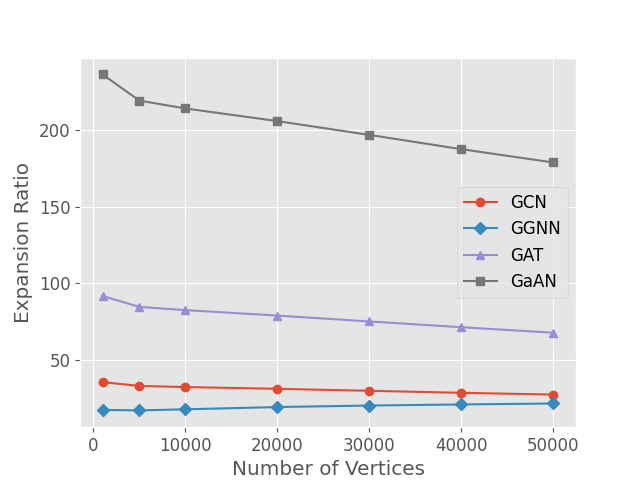
\includegraphics[height=4cm]{figs/experiments/exp_memory_expansion_ratio_input_graph_number_of_vertices_fixed_edge_expansion_ratio.png}}
    \caption{Memory usage changes with the number of graph vertices (R-MAT random graph, the number of edges is fixed at 500k, and the input feature vector dimension is 32)}
    \label{fig:exp_memory_expansion_ratio_input_graph_number_of_vertices_fixed_edge}
\end{figure}

\paragraph{Bottleneck restricting data scalability}
\begin{itemize}
    \item \textbf{GPU memory capacity is the decisive factor limiting the scalability of the training dataset}.
    \item \textbf{GPU memory usage mainly comes from the intermediate calculation results generated during the calculation process,
              especially the intermediate calculation results of the edge calculation. Because part of the intermediate calculation results
              will be cached to participate in backward calculation, high GPU memory usage runs through the forward and backward stages.}
    \item \textbf{GNN's peak memory usage during training can reach tens or even hundreds of times the size of the input data. The limited memory capacity of the GPU severely limits the size of the input data that can be trained}.
    \item \textbf{In the case of a fixed number of vertices, The peak memory usage of GNN increases linearly with the increase of the number of edges of the graph, The proportion of memory expansion will gradually stabilize to a fixed value determined by the complexity of the edge calculation}.
    \item \textbf{In the case where the network structure and various hyperparameters are fixed, using a higher-dimensional input feature vector can reduce the expansion ratio of GPU memory usage}.
\end{itemize}

\label{sec:memory_usage_analysis}
\subsection{Effects of Sampling Techniques on Performance}

Before the sampling technique, GNN training is full batch, that is, all the vertices and edges in the training set participate in the training and calculate the gradient at the same time.
Full batch training can ensure convergence, but the training overhead is large each time, resulting in slow convergence.
Inspired by the minibatch training method in stochastic gradient descent, a series of GNN sampling techniques are proposed.
The sampling technique decomposes the training of the full graph (i.e. epoch) into several batches, and
each batch uses only part of the graph vertices and edges to participate training and performing gradient
updates greatly reduces the training time of each batch, allowing multiple rounds of gradient descent to
be performed within a fixed time, thereby accelerating convergence. The experiments in this section mainly
analyze the impact of sampling techniques on training performance.

In the current implementation of PyG, the GNN model parameters always reside on the GPU,
and the dataset resides in the main memory. When processing each epoch, the CPU samples
the graph dataset in the main memory and generates several batches,
Each batch is a small-scale subgraph of the dataset. When training each batch,
PyG copies the subgraph data corresponding to the batch to the GPU's memory,
trains based on the subgraph and updates the model parameters according to the gradient.
Based on the sampling technology and SGD optimization technology,
the evaluation of the model parameters is performed every several epochs.
The evaluation can be carried out on the CPU or on the GPU.
Therefore, the statistical data in the experiments in this section does not include the evaluation phase.
Neighbor Sampler and Cluster Sampler is selected in this section as they are two typical graph sampling techniques for analysis.

\figurename~\ref{fig:exp_sampling_minibatch_graph_info} shows how the size of the subgraph sampled in the two sampling techniques varies with the batch size.
For Neighbor Sampler, the relative batch size is equal to the number of vertices sampled in the last layer of GNN relative to the top of the full graph the proportion of vertices.
For Cluster Sampler, the batch size is equal to the number of partitions sampled compared to the number of all partitions in the whole graph.
\textbf{Neighbor Sampler is very sensitive to the increase in batch size. As the batch size increases,
    the sampling subgraph The number of vertices/edges and the average degree both increase rapidly and tend to stabilize}.
\textbf{Cluster Sampler is less sensitive to the increase in batch size, the number of vertices/average degree increases
    linearly with the increase in batch size, and the number of edges is in the batch When the size is relatively small,
    it also increases linearly.}

It is worth noting that \textbf{the average degree of the subgraph sampled is much lower than the average degree of the whole graph,
    especially when the relative batch size is low}. Taking Neighbor Sampler at a relative batch size of 6\% as an example,
The average degree of the \textit{amp} dataset is 31.1, but the average degree of the sampled subgraph is only 5.8,
which is much lower than the average degree of the full graph.
The average degree of the subgraph sampled by the Cluster Sampler is lower, only 3.0.
\figurename~\ref{fig:exp_sampling_minibatch_degrees_distribution} shows the comparison of the distribution of the sampled subgraph with the original graph.
The vertex dregree distribution of subgraphs sampled by the two sampling techniques is lower than that of the original graph.
The reason is that the degree distribution of vertex in the actual graph dataset follows a power-rate distribution and only a small number of vertices is very high,
which improves the average degree. In the sampling process, because the sampling method will limit the neighborhood size of the vertex, thereby reducing the upper limit of the vertex degree,
so that the average degree drops significantly. Combined with the experimental results in section 4.2, the decrease in the average degree of sampled subgraph will increase the time-consuming
proportion of vertex calculation. For GGNN with high vertex calculation complexity, vertex calculation will replace edge calculation and become a performance bottleneck.

\begin{figure}
    \centering
    \subfloat[Neighbor Sampler]{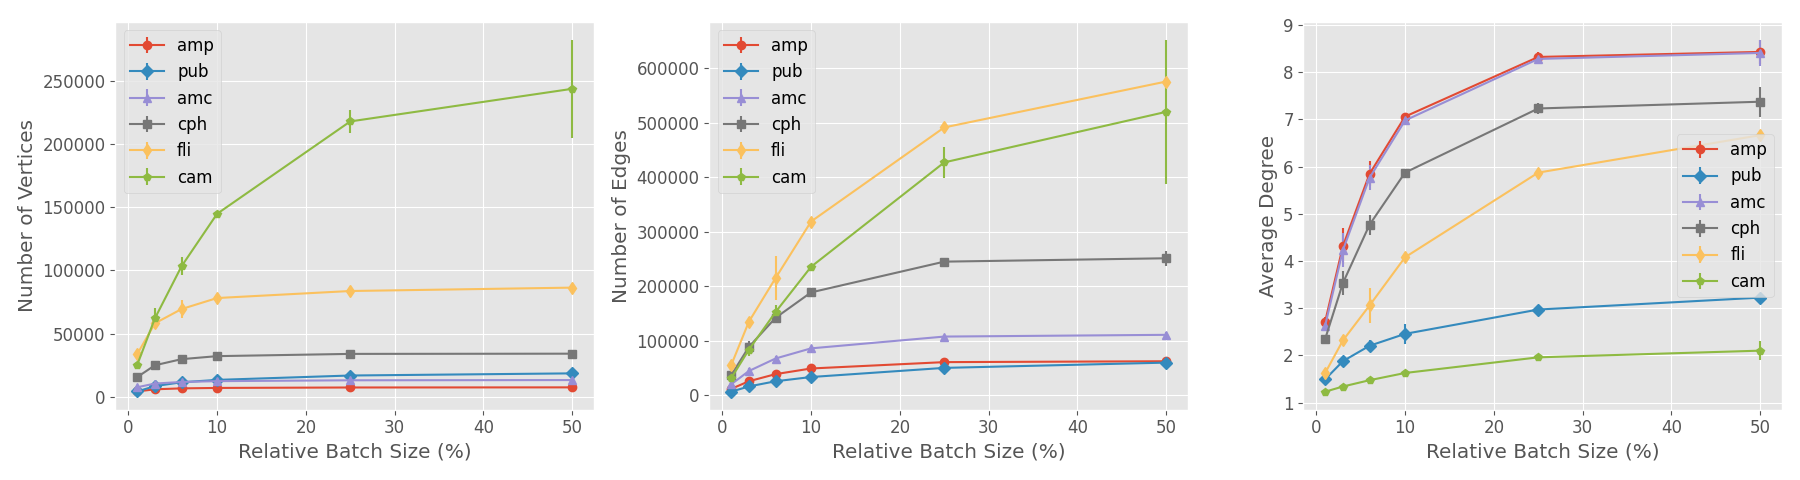
\includegraphics[height=4cm]{figs/experiments/exp_sampling_minibatch_realtive_graph_info_graphsage_gcn.png}} \\
    \subfloat[Cluster Sampler]{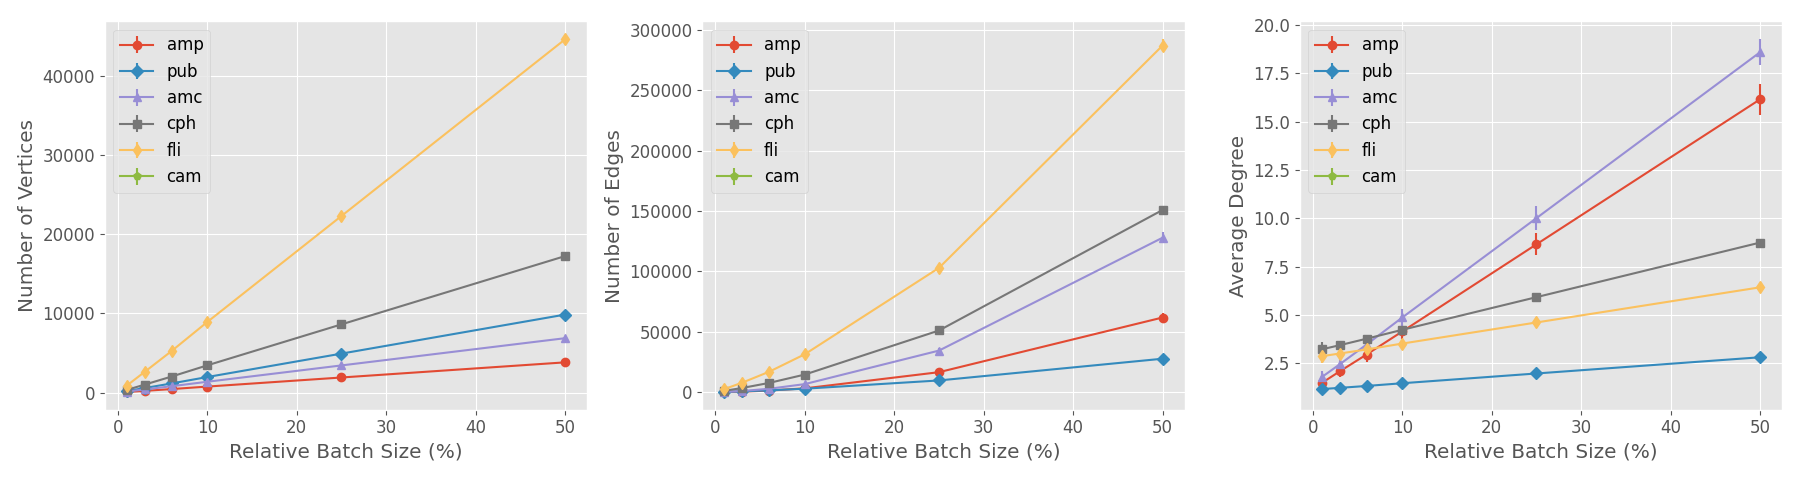
\includegraphics[height=4cm]{figs/experiments/exp_sampling_minibatch_realtive_graph_info_cluster_gcn.png}}
    \caption{The size of the sampled subgraph changes with the batch size. Each batch size is sampled 50 times, and the error bar represents the standard deviation. The relative batch size is the ratio relative to the full graph.)}
    \label{fig:exp_sampling_minibatch_graph_info}
\end{figure}


\begin{figure}
    \centering
    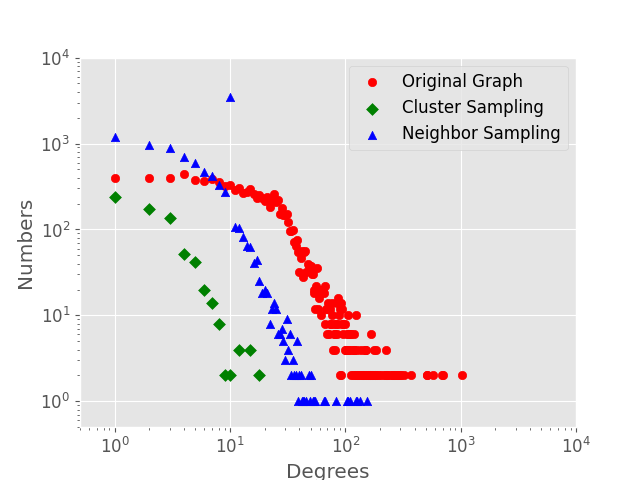
\includegraphics[width=0.7\columnwidth]{figs/experiments/exp_sampling_minibatch_degrees_distribution_amazon-photo.png}
    \caption{Comparison of the vertex degree distribution of the sampled subgraph and the original graph. dataset: amp. Batch size = 512 (Neighbor Sampler) / 20 (Cluster Sampler)}
    \label{fig:exp_sampling_minibatch_degrees_distribution}
\end{figure}

\figurename~\ref{fig:exp_sampling_batch_train_time} shows the change of the training time of each batch on the \textit{amc} and \textit{fli} datasets with the batch size after using the sampling technique.
For the Neighbor Sampler, the time spent in the training phase is significantly reduced compared to full-batch training only when the batch size is very small.
When the batch size is particularly small, the training time is significantly reduced. However, because the sampling itself has additional overhead,
and there is also an overhead in transferring the sampled subgraph to the GPU, the training time of the entire batch may exceed the full graph.
training is time-consuming. For Cluster Sampler, the sampled subgraph is smaller than Neighbor Sampler under the same relative batch size,
which makes the effect of sampling technology more obvious. But when the relative batch size increases,
the increment by additional cost of sampling technology is very obvious. When the relative batch size $\geq$ 25\%,
the total time of each batch of the sampling technique even exceeds the time of the full graph training.
Experiments show that \textbf{the implementation of sampling technology in PyG at this stage is very inefficient and the extra overhead is high}.
When the batch size is slightly larger, the additional cost of sampling technology accounts for more than 50\% of the total training cost of the entire batch.
\textbf{Sampling technology can reduce training time only on very small batches}.

\begin{figure}
    \centering
    \subfloat[Neighbor Sampler on amc]{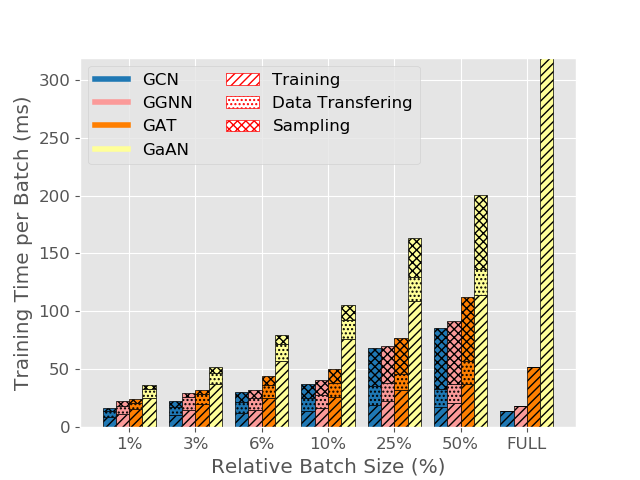
\includegraphics[height=4cm]{figs/experiments/exp_sampling_relative_batch_size_train_time_stack_graphsage_amazon-computers.png}}
    \subfloat[Neighbor Sampler on fli]{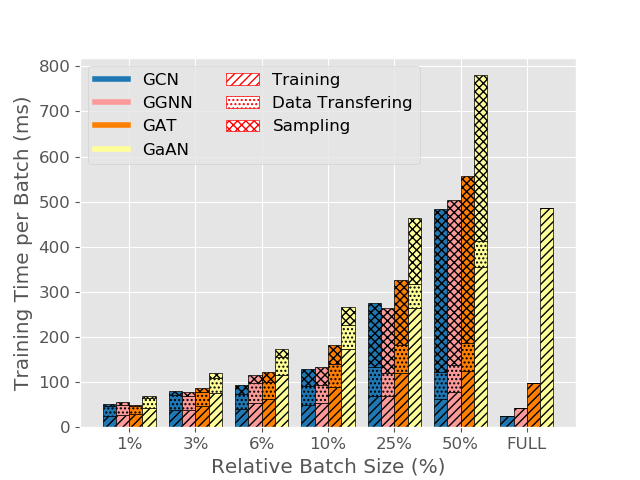
\includegraphics[height=4cm]{figs/experiments/exp_sampling_relative_batch_size_train_time_stack_graphsage_flickr.png}} \\
    \subfloat[Cluster Sampler on amc]{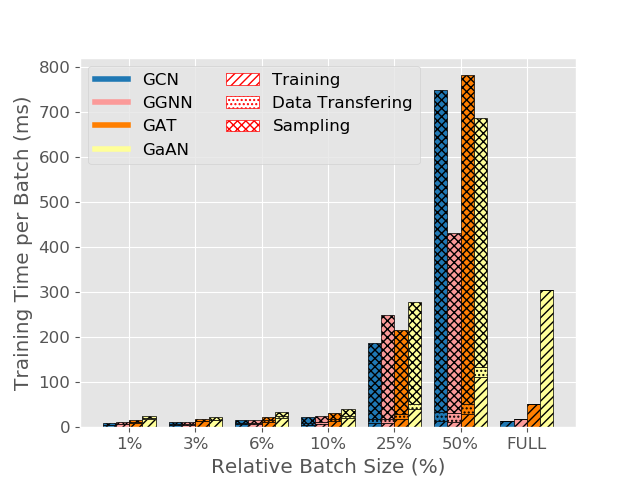
\includegraphics[height=4cm]{figs/experiments/exp_sampling_relative_batch_size_train_time_stack_cluster_amazon-computers.png}}
    \subfloat[Cluster Sampler on fli]{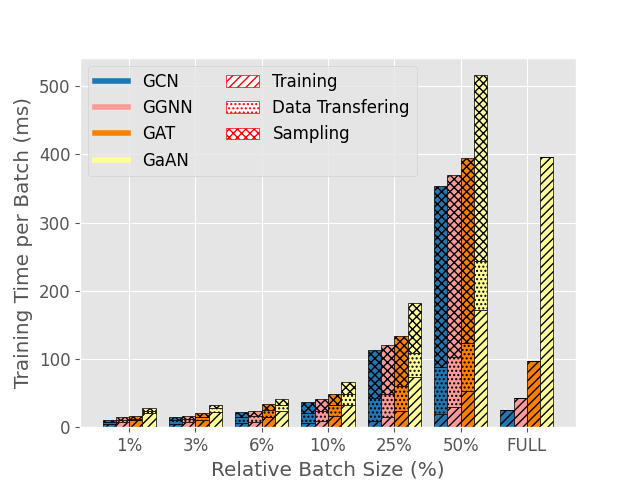
\includegraphics[height=4cm]{figs/experiments/exp_sampling_relative_batch_size_train_time_stack_cluster_flickr.png}}
    \caption{The training time of each batch changes with the batch size. FULL means that the full graph participates in the training phase (excluding evaluation).}
    \label{fig:exp_sampling_batch_train_time}
\end{figure}

However, \textbf{the advantage of the sampling technique is that it can greatly reduce the peak memory usage overhead,
    making large-scale graph neural network training possible}.
\figurename~\ref{fig:exp_sampling_memory_usage} shows how the peak memory usage changes with the relative batch size during the training process after sampling technology is used.
After sampling sampling technology, peak memory usage is greatly reduced and the decrease of Cluster Sampler is greater than that of Neighbor Sampler.

\begin{figure}
    \centering
    \subfloat[Neighbor Sampler on amc]{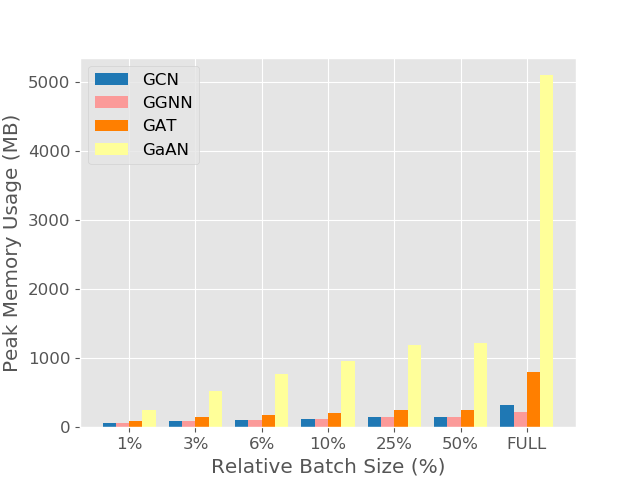
\includegraphics[height=4cm]{figs/experiments/exp_sampling_memory_usage_relative_batch_size_graphsage_amazon-computers_peak_memory.png}}
    \subfloat[Neighbor Sampler on fli]{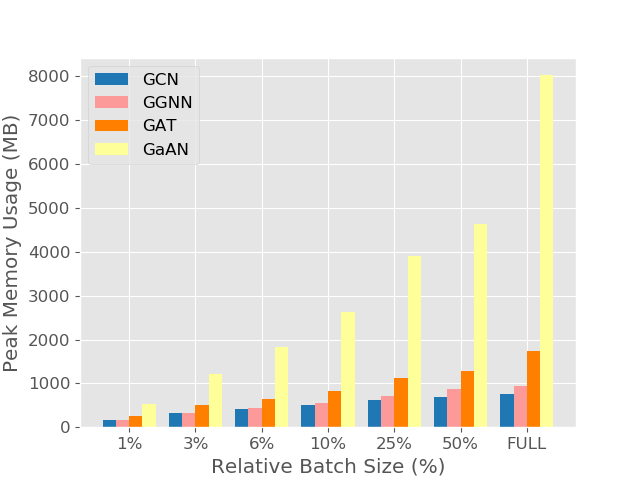
\includegraphics[height=4cm]{figs/experiments/exp_sampling_memory_usage_relative_batch_size_graphsage_flickr_peak_memory.png}} \\
    \subfloat[Cluster Sampler on amc]{\includegraphics[height=4cm]{figs/experiments/exp_sampling_memory_usage_relative_batch_size_cluster_amazon-computers_peak_memory.png}}
    \subfloat[Cluster Sampler on fli]{\includegraphics[height=4cm]{figs/experiments/exp_sampling_memory_usage_relative_batch_size_cluster_flickr_peak_memory.png}}
    \caption{Change in peak memory usage with batch size. FULL indicates the case when the sampling technique is not used (excluding the evaluation stage).}
    \label{fig:exp_sampling_memory_usage}
\end{figure}
\label{sec:effects_of_sampling_techniques_on_performance}
